% Options for packages loaded elsewhere
\PassOptionsToPackage{unicode}{hyperref}
\PassOptionsToPackage{hyphens}{url}
%
\documentclass[
]{book}
\usepackage{amsmath,amssymb}
\usepackage{lmodern}
\usepackage{ifxetex,ifluatex}
\ifnum 0\ifxetex 1\fi\ifluatex 1\fi=0 % if pdftex
  \usepackage[T1]{fontenc}
  \usepackage[utf8]{inputenc}
  \usepackage{textcomp} % provide euro and other symbols
\else % if luatex or xetex
  \usepackage{unicode-math}
  \defaultfontfeatures{Scale=MatchLowercase}
  \defaultfontfeatures[\rmfamily]{Ligatures=TeX,Scale=1}
\fi
% Use upquote if available, for straight quotes in verbatim environments
\IfFileExists{upquote.sty}{\usepackage{upquote}}{}
\IfFileExists{microtype.sty}{% use microtype if available
  \usepackage[]{microtype}
  \UseMicrotypeSet[protrusion]{basicmath} % disable protrusion for tt fonts
}{}
\makeatletter
\@ifundefined{KOMAClassName}{% if non-KOMA class
  \IfFileExists{parskip.sty}{%
    \usepackage{parskip}
  }{% else
    \setlength{\parindent}{0pt}
    \setlength{\parskip}{6pt plus 2pt minus 1pt}}
}{% if KOMA class
  \KOMAoptions{parskip=half}}
\makeatother
\usepackage{xcolor}
\IfFileExists{xurl.sty}{\usepackage{xurl}}{} % add URL line breaks if available
\IfFileExists{bookmark.sty}{\usepackage{bookmark}}{\usepackage{hyperref}}
\hypersetup{
  pdftitle={Book's title},
  pdfauthor={J. Renato Leripio},
  hidelinks,
  pdfcreator={LaTeX via pandoc}}
\urlstyle{same} % disable monospaced font for URLs
\usepackage{color}
\usepackage{fancyvrb}
\newcommand{\VerbBar}{|}
\newcommand{\VERB}{\Verb[commandchars=\\\{\}]}
\DefineVerbatimEnvironment{Highlighting}{Verbatim}{commandchars=\\\{\}}
% Add ',fontsize=\small' for more characters per line
\usepackage{framed}
\definecolor{shadecolor}{RGB}{248,248,248}
\newenvironment{Shaded}{\begin{snugshade}}{\end{snugshade}}
\newcommand{\AlertTok}[1]{\textcolor[rgb]{0.94,0.16,0.16}{#1}}
\newcommand{\AnnotationTok}[1]{\textcolor[rgb]{0.56,0.35,0.01}{\textbf{\textit{#1}}}}
\newcommand{\AttributeTok}[1]{\textcolor[rgb]{0.77,0.63,0.00}{#1}}
\newcommand{\BaseNTok}[1]{\textcolor[rgb]{0.00,0.00,0.81}{#1}}
\newcommand{\BuiltInTok}[1]{#1}
\newcommand{\CharTok}[1]{\textcolor[rgb]{0.31,0.60,0.02}{#1}}
\newcommand{\CommentTok}[1]{\textcolor[rgb]{0.56,0.35,0.01}{\textit{#1}}}
\newcommand{\CommentVarTok}[1]{\textcolor[rgb]{0.56,0.35,0.01}{\textbf{\textit{#1}}}}
\newcommand{\ConstantTok}[1]{\textcolor[rgb]{0.00,0.00,0.00}{#1}}
\newcommand{\ControlFlowTok}[1]{\textcolor[rgb]{0.13,0.29,0.53}{\textbf{#1}}}
\newcommand{\DataTypeTok}[1]{\textcolor[rgb]{0.13,0.29,0.53}{#1}}
\newcommand{\DecValTok}[1]{\textcolor[rgb]{0.00,0.00,0.81}{#1}}
\newcommand{\DocumentationTok}[1]{\textcolor[rgb]{0.56,0.35,0.01}{\textbf{\textit{#1}}}}
\newcommand{\ErrorTok}[1]{\textcolor[rgb]{0.64,0.00,0.00}{\textbf{#1}}}
\newcommand{\ExtensionTok}[1]{#1}
\newcommand{\FloatTok}[1]{\textcolor[rgb]{0.00,0.00,0.81}{#1}}
\newcommand{\FunctionTok}[1]{\textcolor[rgb]{0.00,0.00,0.00}{#1}}
\newcommand{\ImportTok}[1]{#1}
\newcommand{\InformationTok}[1]{\textcolor[rgb]{0.56,0.35,0.01}{\textbf{\textit{#1}}}}
\newcommand{\KeywordTok}[1]{\textcolor[rgb]{0.13,0.29,0.53}{\textbf{#1}}}
\newcommand{\NormalTok}[1]{#1}
\newcommand{\OperatorTok}[1]{\textcolor[rgb]{0.81,0.36,0.00}{\textbf{#1}}}
\newcommand{\OtherTok}[1]{\textcolor[rgb]{0.56,0.35,0.01}{#1}}
\newcommand{\PreprocessorTok}[1]{\textcolor[rgb]{0.56,0.35,0.01}{\textit{#1}}}
\newcommand{\RegionMarkerTok}[1]{#1}
\newcommand{\SpecialCharTok}[1]{\textcolor[rgb]{0.00,0.00,0.00}{#1}}
\newcommand{\SpecialStringTok}[1]{\textcolor[rgb]{0.31,0.60,0.02}{#1}}
\newcommand{\StringTok}[1]{\textcolor[rgb]{0.31,0.60,0.02}{#1}}
\newcommand{\VariableTok}[1]{\textcolor[rgb]{0.00,0.00,0.00}{#1}}
\newcommand{\VerbatimStringTok}[1]{\textcolor[rgb]{0.31,0.60,0.02}{#1}}
\newcommand{\WarningTok}[1]{\textcolor[rgb]{0.56,0.35,0.01}{\textbf{\textit{#1}}}}
\usepackage{longtable,booktabs,array}
\usepackage{calc} % for calculating minipage widths
% Correct order of tables after \paragraph or \subparagraph
\usepackage{etoolbox}
\makeatletter
\patchcmd\longtable{\par}{\if@noskipsec\mbox{}\fi\par}{}{}
\makeatother
% Allow footnotes in longtable head/foot
\IfFileExists{footnotehyper.sty}{\usepackage{footnotehyper}}{\usepackage{footnote}}
\makesavenoteenv{longtable}
\usepackage{graphicx}
\makeatletter
\def\maxwidth{\ifdim\Gin@nat@width>\linewidth\linewidth\else\Gin@nat@width\fi}
\def\maxheight{\ifdim\Gin@nat@height>\textheight\textheight\else\Gin@nat@height\fi}
\makeatother
% Scale images if necessary, so that they will not overflow the page
% margins by default, and it is still possible to overwrite the defaults
% using explicit options in \includegraphics[width, height, ...]{}
\setkeys{Gin}{width=\maxwidth,height=\maxheight,keepaspectratio}
% Set default figure placement to htbp
\makeatletter
\def\fps@figure{htbp}
\makeatother
\setlength{\emergencystretch}{3em} % prevent overfull lines
\providecommand{\tightlist}{%
  \setlength{\itemsep}{0pt}\setlength{\parskip}{0pt}}
\setcounter{secnumdepth}{5}
\usepackage{booktabs}
\ifluatex
  \usepackage{selnolig}  % disable illegal ligatures
\fi
\usepackage[]{natbib}
\bibliographystyle{apalike}

\title{Book's title}
\usepackage{etoolbox}
\makeatletter
\providecommand{\subtitle}[1]{% add subtitle to \maketitle
  \apptocmd{\@title}{\par {\large #1 \par}}{}{}
}
\makeatother
\subtitle{Book's subtitle}
\author{J. Renato Leripio}
\date{2022-02-01}

\begin{document}
\maketitle

{
\setcounter{tocdepth}{1}
\tableofcontents
}
\hypertarget{intro}{%
\chapter{Introduction}\label{intro}}

We will start this book by proposing some short yet very comprehensive exercises on the basics of data wrangling. However, this is by no means an easy or simple task. Since we spend a large portion of our time just cleaning and tidying up the datasets, doing the basics as readable and as efficient as possible is of great value.

\hypertarget{tidyverse}{%
\chapter{The basics of Tidyverse}\label{tidyverse}}

The purpose of this chapter is to introduce the main functions of the core packages in tidyverse. It's not intended to be a thorough description of every function, rather the idea is to provide the basic tools so that those who are either base R users or aren't R users at all can follow along with the rest of the book. For a more detailed approach to tidyverse, the best source is \href{https://r4ds.had.co.nz/}{R for Data Science} by Hadley Wickham \& Garrett Grolemund. For those who feel comfortable with tidyverse, a quick skim through the chapter might be enough.

\hypertarget{whats-tidyverse}{%
\section{What's tidyverse?}\label{whats-tidyverse}}

To start, what's tidyverse? According to the \href{https://www.tidyverse.org/}{official website}:

\begin{quote}
The tidyverse is an opinionated collection of R packages designed for data science. All packages share an underlying design philosophy, grammar, and data structures.
\end{quote}

From my own experience I can ensure you that tidyverse is all you need to carry out data analyses as \textbf{neat}, \textbf{flexible} and \textbf{readable} as possible. By the way, I believe these are the three most important goals for those who want to thrive as a data scientist.

By \textbf{neat} I mean succinct code without any redundancy, a single block of code (not a bunch of loose objects) doing all the desired task. \textbf{Flexible}, in turn, means the code is general enough. It depends on the nature of the task at hand, so take it more like a philosophy. For example, does the solution still work if the data was updated with new values? Does it depend either on column names or the specific length of the vector? Finally, \textbf{readable} means that not only the understanding of the code is easy, but also that it's straightforward to make adjustments to it if necessary.

Most of the time writing neat, flexible and readable code takes longer and requires a dose of creativity, but it surely pays off. Moreover, with practice this will become more and more natural and the cost will get significantly lower.

In the next sections we'll review the most used functions to go through all the steps of everyday data analyses using core tidyverse packages designed to \textbf{Import}, \textbf{Wrangle}, \textbf{Program} and \textbf{Plot}.

\hypertarget{import}{%
\section{Import}\label{import}}

\hypertarget{reading-from-files}{%
\subsection{Reading from files}\label{reading-from-files}}

\texttt{readr} is the package used to import data from flat files (CSV and TXT). The most generic function is \texttt{read\_delim} as it has a large set of arguments that allow us to declare the structure of the data we want to import. In practice, we often use the \texttt{read\_csv} which is a special case of the former with some predefined settings suitable for CSV files -- the most obvious being the comma as the column delimiter.

If you're running RStudio IDE, I recommend you to click on \textbf{Import Dataset} at the \textbf{Environment} sheet (by default it's located in the upper right panel) to manually define the appropriate settings for your file. \textbf{We should never be encouraged to use windows, click on buttons or any kind of shortcuts provided by the IDE. This is the only exception I think is worth it}. First, because it can be tedious to set many specific parameters via trial-and-error to correctly import your data. Second, because once you have the configuration done the code is displayed at the bottom of the window so you can copy it and paste it on your script and, eventually, get rid of this shortcut as you learn how things work. Lastly, you'll usually import one single data set for each task and there's not much to improve on this process. Then, Yes, it's a big waste of time trying to understand each single argument.

Just for the sake of illustration, let's use \texttt{readr} to import the COVID data from Our World in Data we'll use in Chapter \ref{owidCovid}. It's a standard CSV file, so we can use \texttt{read\_csv} without any additional parameter. We just need to provide the file path or URL:

\begin{Shaded}
\begin{Highlighting}[]
\NormalTok{data\_url }\OtherTok{\textless{}{-}} \StringTok{\textquotesingle{}https://raw.githubusercontent.com/owid/covid{-}19{-}data/master/public/data/owid{-}covid{-}data.csv\textquotesingle{}}
\NormalTok{covid\_data\_from\_url   }\OtherTok{\textless{}{-}}\NormalTok{ readr}\SpecialCharTok{::}\FunctionTok{read\_csv}\NormalTok{(data\_url)}
\NormalTok{covid\_data\_from\_local }\OtherTok{\textless{}{-}}\NormalTok{ readr}\SpecialCharTok{::}\FunctionTok{read\_csv}\NormalTok{(}\StringTok{\textquotesingle{}data/owid{-}covid{-}data.csv\textquotesingle{}}\NormalTok{)}
\end{Highlighting}
\end{Shaded}

Tidyverse also provides packages for reading other usual file types. For instance, we can use \texttt{readxl} to read MS Excel spreadsheets and \texttt{haven} to read data generated by popular statistical softwares (SPSS, Stata and SAS) in much the same way we did with \texttt{readr} for CSV files -- you can check them at the \textbf{Import Dataset} dropdown menu. So we won't waste time covering them. Rather, let's use the rest of this section to talk about something very important and that usually gets less attention in books.

\hypertarget{reading-from-api}{%
\subsection{Reading from API}\label{reading-from-api}}

Although the use of these traditional file formats are still widespread, organizations are increasingly switching to API's to make data available to the public. This is a huge improvement since we're able to customize our demand and retrieve only the data we need for the specific task.

If you don't know what an API is, think of it as an interface to establish a connection to a database. However, instead of reading all the content from this database you can inform your \textbf{preferences} like what columns you want, the desired observations (time range if it's a time series) and so on. These preferences are embedded in a \textbf{request} and the right form to specify it is usually available in a documentation provided by the API maintainer.

For example, the Federal Reserve Bank of St.~Louis maintains a huge repository with hundreds of thousands of economic time series and we can import them using an API. The information on how to build the request is available in the \href{https://fred.stlouisfed.org/docs/api/fred/}{documentation}, where we can see a link with instructions on how to \textbf{`Get the observations or data values for an economic data series'}. There, we find an example of a request for the US Real Gross National Product:

\url{https://api.stlouisfed.org/fred/series/observations?series_id=GNPCA\&api_key=abcdefghijklmnopqrstuvwxyz123456\&file_type=json}

We can break this request to see its parts in more detail:

\begin{enumerate}
\def\labelenumi{\arabic{enumi}.}
\tightlist
\item
  The static URL to access the \textbf{Observations} section in the API.
\end{enumerate}

\$ \underbrace{\text{https://api.stlouisfed.org/fred/series/observations?}}\_\text{Static: API URL} \$

\begin{enumerate}
\def\labelenumi{\arabic{enumi}.}
\setcounter{enumi}{1}
\tightlist
\item
  The series ID which identifies what series we want.
\end{enumerate}

\$ \underbrace{\text{series_id=GNPCA}}\_\text{Param. #1: Series ID} \$

\begin{enumerate}
\def\labelenumi{\arabic{enumi}.}
\setcounter{enumi}{2}
\tightlist
\item
  The API Key. We must create an account and require a personal key in order to retrieve data from the API. This one is an example for illustrative purposes only.
\end{enumerate}

\$ \underbrace{\text{api_key=abcdefghijklmnopqrstuvwxyz123456}}\_\text{Param. #2: API Key} \$

\begin{enumerate}
\def\labelenumi{\arabic{enumi}.}
\setcounter{enumi}{3}
\tightlist
\item
  The file type for the output. There are several types, but I'd rather working with JSON.
\end{enumerate}

\$ \underbrace{\text{file_type=json}}\_\text{Param. #3: File Type} \$

Note that all the parameters following the static part is separated by an \textbf{\&}. Then, if we want to add any extra parameter it should be placed right after an \textbf{\&}.

Suppose we want to read monthly data for the \href{https://fred.stlouisfed.org/series/CPALTT01USM657N}{US Consumer Price Index (CPI)}. The \texttt{series\_id} is \textbf{CPALTT01USM657N}. Besides, we'd only like to read data as of January 2010. How can we do so? There's a parameter \texttt{observation\_start} which defines the start of the observation period (YYYY-MM-DD format).

The code below creates a separate object for each part of the request. Then, we use the \texttt{glue} function from the homonymous package to merge the pieces into a single string adding the appropriate \textbf{\&}. Of course, we could create the complete string all at once. But, creating separate objects makes it easier to find and edit values as well as to transform this task into a function if we had to read other data from this source frequently (more on this later in Chapter \ref{google}).

\begin{Shaded}
\begin{Highlighting}[]
\NormalTok{api\_url       }\OtherTok{\textless{}{-}} \StringTok{\textquotesingle{}https://api.stlouisfed.org/fred/series/observations?\textquotesingle{}}
\NormalTok{api\_key       }\OtherTok{\textless{}{-}} \StringTok{\textquotesingle{}bc0b91e1c6fa2cab4d4f180c7965edfa\textquotesingle{}}
\NormalTok{api\_series\_id }\OtherTok{\textless{}{-}} \StringTok{\textquotesingle{}CPALTT01USM657N\textquotesingle{}}
\NormalTok{obs\_start     }\OtherTok{\textless{}{-}} \StringTok{\textquotesingle{}2010{-}01{-}01\textquotesingle{}}
\NormalTok{api\_filetype  }\OtherTok{\textless{}{-}} \StringTok{\textquotesingle{}json\textquotesingle{}}
\NormalTok{api\_request   }\OtherTok{\textless{}{-}}\NormalTok{ glue}\SpecialCharTok{::}\FunctionTok{glue}\NormalTok{(}\StringTok{\textquotesingle{}\{api\_url\}series\_id=\{api\_series\_id\}\&observation\_start=\{obs\_start\}\&api\_key=\{api\_key\}\&file\_type=\{api\_filetype\}\textquotesingle{}}\NormalTok{)}
\end{Highlighting}
\end{Shaded}

Now, we use the \texttt{httr} package to connect to the API, send the request and get the content. The other steps transform the content from JSON to a standard R object (a list) and then convert it to a tibble (the tidyverse's improved format for data frames). The element \texttt{observations} is specific for this API, so if we imported data from another source we'd have to check in which element the desired content would be stored.

\begin{Shaded}
\begin{Highlighting}[]
\FunctionTok{library}\NormalTok{(magrittr)}
\NormalTok{cpi\_request }\OtherTok{\textless{}{-}}\NormalTok{ httr}\SpecialCharTok{::}\FunctionTok{GET}\NormalTok{(}\AttributeTok{url =}\NormalTok{ api\_request)}
\NormalTok{cpi\_content }\OtherTok{\textless{}{-}}\NormalTok{ httr}\SpecialCharTok{::}\FunctionTok{content}\NormalTok{(cpi\_request, }\AttributeTok{as =} \StringTok{\textquotesingle{}text\textquotesingle{}}\NormalTok{)}
\NormalTok{cpi\_list    }\OtherTok{\textless{}{-}}\NormalTok{ jsonlite}\SpecialCharTok{::}\FunctionTok{fromJSON}\NormalTok{(cpi\_content, }\AttributeTok{flatten =} \ConstantTok{FALSE}\NormalTok{)}
\NormalTok{cpi\_tbl     }\OtherTok{\textless{}{-}}\NormalTok{ cpi\_list[[}\StringTok{\textquotesingle{}observations\textquotesingle{}}\NormalTok{]] }\SpecialCharTok{\%\textgreater{}\%}\NormalTok{ tibble}\SpecialCharTok{::}\FunctionTok{as\_tibble}\NormalTok{()}
\NormalTok{cpi\_tbl}
\end{Highlighting}
\end{Shaded}

\begin{verbatim}
## # A tibble: 144 x 4
##    realtime_start realtime_end date       value              
##    <chr>          <chr>        <chr>      <chr>              
##  1 2022-02-01     2022-02-01   2010-01-01 0.34174735701485   
##  2 2022-02-01     2022-02-01   2010-02-01 0.024920738207648  
##  3 2022-02-01     2022-02-01   2010-03-01 0.410628353657108  
##  4 2022-02-01     2022-02-01   2010-04-01 0.173688491069743  
##  5 2022-02-01     2022-02-01   2010-05-01 0.0775197354237721 
##  6 2022-02-01     2022-02-01   2010-06-01 -0.0976267084673888
##  7 2022-02-01     2022-02-01   2010-07-01 0.0211043057371509 
##  8 2022-02-01     2022-02-01   2010-08-01 0.138066427840807  
##  9 2022-02-01     2022-02-01   2010-09-01 0.0581736230715569 
## 10 2022-02-01     2022-02-01   2010-10-01 0.124519888847696  
## # ... with 134 more rows
\end{verbatim}

This concludes our section on how to import data. If you're struggling with other types of data, Tidyverse's official \href{https://www.tidyverse.org/packages/\#import}{website} provides a comprehensive list of all the supported file formats and the respective packages used to handle them.

\hypertarget{wrangle}{%
\section{Wrangle}\label{wrangle}}

This is by far the most important section in this Chapter. The main goal here is to provide a general sense of how to get raw data ready to use. For this, we'll focus on the roles of the main functions inside the core packages rather than the idiosyncrasies and generalizations of each one. A deeper approach will be taken in the next chapters.

\hypertarget{data-manipulation}{%
\subsection{Data manipulation}\label{data-manipulation}}

Let's use the COVID data we read in the last section. Starting with the \texttt{glimpse} function to have a grasp of the data, we can see some useful information such as the number of rows and columns, as well as columns' names and classes (whether they're character, double, etc).

\begin{Shaded}
\begin{Highlighting}[]
\NormalTok{covid\_data }\OtherTok{\textless{}{-}}\NormalTok{ readr}\SpecialCharTok{::}\FunctionTok{read\_csv}\NormalTok{(}\StringTok{\textquotesingle{}data/owid{-}covid{-}data.csv\textquotesingle{}}\NormalTok{)}
\NormalTok{covid\_data }\SpecialCharTok{\%\textgreater{}\%} 
\NormalTok{  dplyr}\SpecialCharTok{::}\FunctionTok{glimpse}\NormalTok{()}
\end{Highlighting}
\end{Shaded}

\begin{verbatim}
## Rows: 148,800
## Columns: 67
## $ iso_code                                   <chr> "AFG", "AFG", "AFG", "AFG",~
## $ continent                                  <chr> "Asia", "Asia", "Asia", "As~
## $ location                                   <chr> "Afghanistan", "Afghanistan~
## $ date                                       <date> 2020-02-24, 2020-02-25, 20~
## $ total_cases                                <dbl> 5, 5, 5, 5, 5, 5, 5, 5, 5, ~
## $ new_cases                                  <dbl> 5, 0, 0, 0, 0, 0, 0, 0, 0, ~
## $ new_cases_smoothed                         <dbl> NA, NA, NA, NA, NA, 0.714, ~
## $ total_deaths                               <dbl> NA, NA, NA, NA, NA, NA, NA,~
## $ new_deaths                                 <dbl> NA, NA, NA, NA, NA, NA, NA,~
## $ new_deaths_smoothed                        <dbl> NA, NA, NA, NA, NA, 0, 0, 0~
## $ total_cases_per_million                    <dbl> 0.126, 0.126, 0.126, 0.126,~
## $ new_cases_per_million                      <dbl> 0.126, 0.000, 0.000, 0.000,~
## $ new_cases_smoothed_per_million             <dbl> NA, NA, NA, NA, NA, 0.018, ~
## $ total_deaths_per_million                   <dbl> NA, NA, NA, NA, NA, NA, NA,~
## $ new_deaths_per_million                     <dbl> NA, NA, NA, NA, NA, NA, NA,~
## $ new_deaths_smoothed_per_million            <dbl> NA, NA, NA, NA, NA, 0, 0, 0~
## $ reproduction_rate                          <dbl> NA, NA, NA, NA, NA, NA, NA,~
## $ icu_patients                               <dbl> NA, NA, NA, NA, NA, NA, NA,~
## $ icu_patients_per_million                   <dbl> NA, NA, NA, NA, NA, NA, NA,~
## $ hosp_patients                              <dbl> NA, NA, NA, NA, NA, NA, NA,~
## $ hosp_patients_per_million                  <dbl> NA, NA, NA, NA, NA, NA, NA,~
## $ weekly_icu_admissions                      <dbl> NA, NA, NA, NA, NA, NA, NA,~
## $ weekly_icu_admissions_per_million          <dbl> NA, NA, NA, NA, NA, NA, NA,~
## $ weekly_hosp_admissions                     <dbl> NA, NA, NA, NA, NA, NA, NA,~
## $ weekly_hosp_admissions_per_million         <dbl> NA, NA, NA, NA, NA, NA, NA,~
## $ new_tests                                  <dbl> NA, NA, NA, NA, NA, NA, NA,~
## $ total_tests                                <dbl> NA, NA, NA, NA, NA, NA, NA,~
## $ total_tests_per_thousand                   <dbl> NA, NA, NA, NA, NA, NA, NA,~
## $ new_tests_per_thousand                     <dbl> NA, NA, NA, NA, NA, NA, NA,~
## $ new_tests_smoothed                         <dbl> NA, NA, NA, NA, NA, NA, NA,~
## $ new_tests_smoothed_per_thousand            <dbl> NA, NA, NA, NA, NA, NA, NA,~
## $ positive_rate                              <dbl> NA, NA, NA, NA, NA, NA, NA,~
## $ tests_per_case                             <dbl> NA, NA, NA, NA, NA, NA, NA,~
## $ tests_units                                <chr> NA, NA, NA, NA, NA, NA, NA,~
## $ total_vaccinations                         <dbl> NA, NA, NA, NA, NA, NA, NA,~
## $ people_vaccinated                          <dbl> NA, NA, NA, NA, NA, NA, NA,~
## $ people_fully_vaccinated                    <dbl> NA, NA, NA, NA, NA, NA, NA,~
## $ total_boosters                             <dbl> NA, NA, NA, NA, NA, NA, NA,~
## $ new_vaccinations                           <dbl> NA, NA, NA, NA, NA, NA, NA,~
## $ new_vaccinations_smoothed                  <dbl> NA, NA, NA, NA, NA, NA, NA,~
## $ total_vaccinations_per_hundred             <dbl> NA, NA, NA, NA, NA, NA, NA,~
## $ people_vaccinated_per_hundred              <dbl> NA, NA, NA, NA, NA, NA, NA,~
## $ people_fully_vaccinated_per_hundred        <dbl> NA, NA, NA, NA, NA, NA, NA,~
## $ total_boosters_per_hundred                 <dbl> NA, NA, NA, NA, NA, NA, NA,~
## $ new_vaccinations_smoothed_per_million      <dbl> NA, NA, NA, NA, NA, NA, NA,~
## $ new_people_vaccinated_smoothed             <dbl> NA, NA, NA, NA, NA, NA, NA,~
## $ new_people_vaccinated_smoothed_per_hundred <dbl> NA, NA, NA, NA, NA, NA, NA,~
## $ stringency_index                           <dbl> 8.33, 8.33, 8.33, 8.33, 8.3~
## $ population                                 <dbl> 39835428, 39835428, 3983542~
## $ population_density                         <dbl> 54.422, 54.422, 54.422, 54.~
## $ median_age                                 <dbl> 18.6, 18.6, 18.6, 18.6, 18.~
## $ aged_65_older                              <dbl> 2.581, 2.581, 2.581, 2.581,~
## $ aged_70_older                              <dbl> 1.337, 1.337, 1.337, 1.337,~
## $ gdp_per_capita                             <dbl> 1803.987, 1803.987, 1803.98~
## $ extreme_poverty                            <dbl> NA, NA, NA, NA, NA, NA, NA,~
## $ cardiovasc_death_rate                      <dbl> 597.029, 597.029, 597.029, ~
## $ diabetes_prevalence                        <dbl> 9.59, 9.59, 9.59, 9.59, 9.5~
## $ female_smokers                             <dbl> NA, NA, NA, NA, NA, NA, NA,~
## $ male_smokers                               <dbl> NA, NA, NA, NA, NA, NA, NA,~
## $ handwashing_facilities                     <dbl> 37.746, 37.746, 37.746, 37.~
## $ hospital_beds_per_thousand                 <dbl> 0.5, 0.5, 0.5, 0.5, 0.5, 0.~
## $ life_expectancy                            <dbl> 64.83, 64.83, 64.83, 64.83,~
## $ human_development_index                    <dbl> 0.511, 0.511, 0.511, 0.511,~
## $ excess_mortality_cumulative_absolute       <dbl> NA, NA, NA, NA, NA, NA, NA,~
## $ excess_mortality_cumulative                <dbl> NA, NA, NA, NA, NA, NA, NA,~
## $ excess_mortality                           <dbl> NA, NA, NA, NA, NA, NA, NA,~
## $ excess_mortality_cumulative_per_million    <dbl> NA, NA, NA, NA, NA, NA, NA,~
\end{verbatim}

We're usually not interested in all of these data, so the first couple of tasks we'd like to perform is to filter the relevant categories and select the desired columns. For example, we could be interested in analyzing new COVID cases (column \texttt{new\_cases}) only in Brazil (rows equal to \texttt{Brazil} in column \texttt{location}). Furthermore, we'd like to get rid of duplicate rows if there's any.

One of the great contributions of tidyverse is to assign names to the functions according to the actions they perform -- many are admittedly SQL-inspired. \texttt{distinct} select only unique rows from a data set, thus dropping duplicates. \texttt{select} picks variables based on their names, whereas \texttt{filter} retains the rows which satisfy a given condition -- or a set of conditions.

Conditions are sentences which returns \texttt{TRUE} or \texttt{FALSE}. It's straightforward to think of conditions using logical operators, such as \texttt{==}, \texttt{\textgreater{}}, \texttt{\textless{}}, etc. Nevertheless, there's a bunch of expressions in R which return \texttt{TRUE} or \texttt{FALSE}. Moreover, we can always create our own condition to suit the work purpose. We'll see many examples throughout this book.

We can use the code below to generate the desired subset of the data:

\begin{Shaded}
\begin{Highlighting}[]
\NormalTok{covid\_data\_01 }\OtherTok{\textless{}{-}}\NormalTok{ covid\_data }\SpecialCharTok{\%\textgreater{}\%} 
\NormalTok{  dplyr}\SpecialCharTok{::}\FunctionTok{distinct}\NormalTok{() }\SpecialCharTok{\%\textgreater{}\%} 
\NormalTok{  dplyr}\SpecialCharTok{::}\FunctionTok{select}\NormalTok{(date, continent, location, new\_cases) }\SpecialCharTok{\%\textgreater{}\%} 
\NormalTok{  dplyr}\SpecialCharTok{::}\FunctionTok{filter}\NormalTok{(location }\SpecialCharTok{==} \StringTok{\textquotesingle{}Brazil\textquotesingle{}}\NormalTok{)}
\end{Highlighting}
\end{Shaded}

Next, we'd probably need to create additional columns. For instance, suppose that actual new cases in Brazil are much higher than reported because the country doesn't have enough tests and a conservative estimate points to a number of, at least, twice the official count. So we'd like to add a column which is twice the value of the original one representing our guess of the real situation. In addition, we'd also like to create a column to indicate the dominant strain at each period of time. We know that the Delta strain took over Gamma by the end of July 2021 and, then, Omicron took over Delta in the beginning of 2022.

\texttt{mutate} can be used to create new variables as a function of existing variables, but not necessarily. Also, it can be used to modify existing variables as new variables overwrites existing variables of the same name. \texttt{case\_when} is another SQL-inspired function used inside \texttt{mutate} to create a new variable based on conditions. It's worth noting that it'll return \texttt{NA} if no condition is met. In this case, a useful workaround is to define an extra condition as \texttt{TRUE\ \textasciitilde{}\ value}, thus assigning a value to all the unmet conditions -- think of this as an \textbf{else} condition.

\begin{Shaded}
\begin{Highlighting}[]
\NormalTok{covid\_data\_02 }\OtherTok{\textless{}{-}}\NormalTok{ covid\_data\_01 }\SpecialCharTok{\%\textgreater{}\%} 
\NormalTok{  dplyr}\SpecialCharTok{::}\FunctionTok{mutate}\NormalTok{(}
    \AttributeTok{real\_new\_cases =}\NormalTok{ new\_cases}\SpecialCharTok{*}\DecValTok{2}\NormalTok{,}
    \AttributeTok{dominant\_strain  =}\NormalTok{ dplyr}\SpecialCharTok{::}\FunctionTok{case\_when}\NormalTok{(}
\NormalTok{      date }\SpecialCharTok{\textless{}=} \StringTok{\textquotesingle{}2021{-}07{-}31\textquotesingle{}}                        \SpecialCharTok{\textasciitilde{}} \StringTok{\textquotesingle{}Gamma\textquotesingle{}}\NormalTok{,}
\NormalTok{      date }\SpecialCharTok{\textgreater{}}  \StringTok{\textquotesingle{}2021{-}07{-}31\textquotesingle{}} \SpecialCharTok{\&}\NormalTok{ date }\SpecialCharTok{\textless{}=} \StringTok{\textquotesingle{}2021{-}12{-}31\textquotesingle{}} \SpecialCharTok{\textasciitilde{}} \StringTok{\textquotesingle{}Delta\textquotesingle{}}\NormalTok{,}
\NormalTok{      date }\SpecialCharTok{\textgreater{}}  \StringTok{\textquotesingle{}2021{-}12{-}31\textquotesingle{}} \SpecialCharTok{\&}\NormalTok{ date }\SpecialCharTok{\textless{}=} \StringTok{\textquotesingle{}2022{-}02{-}01\textquotesingle{}} \SpecialCharTok{\textasciitilde{}} \StringTok{\textquotesingle{}Omicron\textquotesingle{}}\NormalTok{,}
      \ConstantTok{TRUE}                                        \SpecialCharTok{\textasciitilde{}} \StringTok{"We don\textquotesingle{}t know"}
\NormalTok{    )}
\NormalTok{  )}
\end{Highlighting}
\end{Shaded}

So far we've worked on a single group of data: new cases in Brazil. However, we usually have many categories to work on. We might be interested in analyzing new cases in all European countries. In this case, we'll need the \texttt{group\_by} function, which allows us to perform any operation by group. \texttt{group\_by} is often used in conjunction with \texttt{mutate} or \texttt{summarise} to create new data for each group. The latter uses aggregate functions (\texttt{mean}, \texttt{max}, \texttt{min}, etc) to produce a summary of the data.

For example, suppose we want to know which European country recorded the highest number of new covid cases in a single day by the end of 2021. This might be achieved by grouping the data by location and then using \texttt{summarise} with \texttt{max}. In addition, we can use \texttt{arrange} to sort the rows by value (we use \texttt{desc} to sort in descending order). Don't forget to \texttt{ungroup} data as soon as you no longer need to perform operations by group.

\begin{Shaded}
\begin{Highlighting}[]
\NormalTok{covid\_data\_03 }\OtherTok{\textless{}{-}}\NormalTok{ covid\_data }\SpecialCharTok{\%\textgreater{}\%} 
\NormalTok{  dplyr}\SpecialCharTok{::}\FunctionTok{distinct}\NormalTok{() }\SpecialCharTok{\%\textgreater{}\%} 
\NormalTok{  dplyr}\SpecialCharTok{::}\FunctionTok{filter}\NormalTok{(continent }\SpecialCharTok{==} \StringTok{\textquotesingle{}Europe\textquotesingle{}}\NormalTok{,}
\NormalTok{                date }\SpecialCharTok{\textless{}=} \StringTok{\textquotesingle{}2021{-}12{-}31\textquotesingle{}}\NormalTok{) }\SpecialCharTok{\%\textgreater{}\%} 
\NormalTok{  dplyr}\SpecialCharTok{::}\FunctionTok{group\_by}\NormalTok{(location) }\SpecialCharTok{\%\textgreater{}\%} 
\NormalTok{  dplyr}\SpecialCharTok{::}\FunctionTok{summarise}\NormalTok{(}\AttributeTok{max\_new\_cases =} \FunctionTok{max}\NormalTok{(new\_cases)) }\SpecialCharTok{\%\textgreater{}\%} 
\NormalTok{  dplyr}\SpecialCharTok{::}\FunctionTok{ungroup}\NormalTok{() }\SpecialCharTok{\%\textgreater{}\%} 
\NormalTok{  dplyr}\SpecialCharTok{::}\FunctionTok{arrange}\NormalTok{(}\FunctionTok{desc}\NormalTok{(max\_new\_cases))}
\end{Highlighting}
\end{Shaded}

Note that some countries such as Spain, Portugal and France returned \texttt{NA}. This happened because they probably have any missing value. We could easily ignore it by passing the argument \texttt{na.rm\ =\ TRUE} to the \texttt{max} function. However, another problem would arise: countries with no data on new cases would return \texttt{-Inf}. To get around these two issues, we can filter out all the missing values in the data set (the \texttt{!} before the condition works as a negation). In this case removing the missing values isn't a problem, but be aware that for some tasks this may influence the outcome.

\begin{Shaded}
\begin{Highlighting}[]
\NormalTok{covid\_data\_04 }\OtherTok{\textless{}{-}}\NormalTok{ covid\_data }\SpecialCharTok{\%\textgreater{}\%} 
\NormalTok{  dplyr}\SpecialCharTok{::}\FunctionTok{distinct}\NormalTok{() }\SpecialCharTok{\%\textgreater{}\%} 
\NormalTok{  dplyr}\SpecialCharTok{::}\FunctionTok{filter}\NormalTok{(continent }\SpecialCharTok{==} \StringTok{\textquotesingle{}Europe\textquotesingle{}}\NormalTok{,}
\NormalTok{                date }\SpecialCharTok{\textless{}=} \StringTok{\textquotesingle{}2021{-}12{-}31\textquotesingle{}}\NormalTok{,}
                \SpecialCharTok{!}\FunctionTok{is.na}\NormalTok{(new\_cases)) }\SpecialCharTok{\%\textgreater{}\%} 
\NormalTok{  dplyr}\SpecialCharTok{::}\FunctionTok{group\_by}\NormalTok{(location) }\SpecialCharTok{\%\textgreater{}\%} 
\NormalTok{  dplyr}\SpecialCharTok{::}\FunctionTok{summarise}\NormalTok{(}\AttributeTok{max\_new\_cases =} \FunctionTok{max}\NormalTok{(new\_cases)) }\SpecialCharTok{\%\textgreater{}\%} 
\NormalTok{  dplyr}\SpecialCharTok{::}\FunctionTok{ungroup}\NormalTok{()}
   
\NormalTok{covid\_data\_04     }
\end{Highlighting}
\end{Shaded}

\begin{verbatim}
## # A tibble: 49 x 2
##    location               max_new_cases
##    <chr>                          <dbl>
##  1 Albania                         1239
##  2 Andorra                          696
##  3 Austria                        15809
##  4 Belarus                         2097
##  5 Belgium                        47836
##  6 Bosnia and Herzegovina          3755
##  7 Bulgaria                        7560
##  8 Croatia                         7315
##  9 Cyprus                          1909
## 10 Czechia                        27793
## # ... with 39 more rows
\end{verbatim}

In addition, we might want to know not only what the highest numbers were but when they did occur (the peak date). Since the \texttt{summarise} function is designed to return a single value, we must use an expression which returns a single value. If we used \texttt{date\ =\ max(date)}, we'd keep the most recent date for the data in each country. Definitely, that's not what we want. So a good way to address this issue is to combine a subset operation with a condition inside. In simpler terms, we'll subset from the column date the observation where new cases were at their high. Since we can have multiple dates which satisfy this condition, we'll keep the most recent one (the \texttt{max} of them).

\begin{Shaded}
\begin{Highlighting}[]
\NormalTok{covid\_data\_05 }\OtherTok{\textless{}{-}}\NormalTok{ covid\_data }\SpecialCharTok{\%\textgreater{}\%} 
\NormalTok{  dplyr}\SpecialCharTok{::}\FunctionTok{distinct}\NormalTok{() }\SpecialCharTok{\%\textgreater{}\%} 
\NormalTok{  dplyr}\SpecialCharTok{::}\FunctionTok{filter}\NormalTok{(continent }\SpecialCharTok{==} \StringTok{\textquotesingle{}Europe\textquotesingle{}}\NormalTok{,}
\NormalTok{                date }\SpecialCharTok{\textless{}=} \StringTok{\textquotesingle{}2021{-}12{-}31\textquotesingle{}}\NormalTok{,}
                \SpecialCharTok{!}\FunctionTok{is.na}\NormalTok{(new\_cases)) }\SpecialCharTok{\%\textgreater{}\%} 
\NormalTok{  dplyr}\SpecialCharTok{::}\FunctionTok{group\_by}\NormalTok{(location) }\SpecialCharTok{\%\textgreater{}\%} 
\NormalTok{  dplyr}\SpecialCharTok{::}\FunctionTok{summarise}\NormalTok{(}\AttributeTok{max\_new\_cases =} \FunctionTok{max}\NormalTok{(new\_cases),}
                   \AttributeTok{peak\_date =}\NormalTok{ date[}\FunctionTok{which}\NormalTok{(new\_cases }\SpecialCharTok{==}\NormalTok{ max\_new\_cases)],}
                   \AttributeTok{peak\_date =} \FunctionTok{max}\NormalTok{(peak\_date)) }\SpecialCharTok{\%\textgreater{}\%} 
\NormalTok{  dplyr}\SpecialCharTok{::}\FunctionTok{ungroup}\NormalTok{() }\SpecialCharTok{\%\textgreater{}\%} 
\NormalTok{  dplyr}\SpecialCharTok{::}\FunctionTok{arrange}\NormalTok{(peak\_date) }\SpecialCharTok{\%\textgreater{}\%} 
\NormalTok{  dplyr}\SpecialCharTok{::}\FunctionTok{slice}\NormalTok{(}\DecValTok{1}\SpecialCharTok{:}\DecValTok{10}\NormalTok{)}
   
\NormalTok{covid\_data\_05   }
\end{Highlighting}
\end{Shaded}

\begin{verbatim}
## # A tibble: 10 x 3
##    location   max_new_cases peak_date 
##    <chr>              <dbl> <date>    
##  1 Vatican                7 2020-10-15
##  2 Vatican                7 2020-10-15
##  3 Luxembourg          1967 2020-11-02
##  4 Montenegro           874 2020-11-04
##  5 Italy              40902 2020-11-13
##  6 Sweden             32485 2020-12-29
##  7 Gibraltar            180 2020-12-30
##  8 Lithuania           3984 2020-12-30
##  9 Ireland             8227 2021-01-08
## 10 Spain              93822 2021-01-25
\end{verbatim}

\begin{Shaded}
\begin{Highlighting}[]
\CommentTok{\# Verificar depois por que Vaticano aparece com 2 entradas}
\end{Highlighting}
\end{Shaded}

In case it went unnoticed, the previous code showed a really nice feature of \texttt{mutate}/\texttt{summarise}: you can use a variable you've just created in a subsequent task inside the same calling. In this example, we used the maximum number of new cases (first variable created) as a reference to obtain the dates when it occurred (second variable created) and them picked only the maximum date from a possibly set of dates (third variable created), all of this inside the same \texttt{summarise} calling as if all steps were performed sequentially.

Finally, we used \texttt{arrange} to sort countries by their peak date (this time by ascending order, the default) and then \texttt{slice} to subset only the first ten countries out of the forty-nine in our data set.

\textbf{Falar dos joins, bind-rows/cols}

\hypertarget{data-layout}{%
\subsection{Data layout}\label{data-layout}}

We've walked through all the main functions of \texttt{dplyr}. Now, we turn to the \texttt{tidyr} package. According to tidyverse's website, the goal of \texttt{tidyr} is to help us create \textbf{tidy data}. It means a data set where every column is a variable; every row is an observation; and each cell is a single value. This is more like a convention created by tidyverse so that \emph{``you'll spend less time fighting with the tools and more time working on your analysis''}.

Tidy data is also known as \textbf{wide} format -- since it increases the number of columns and decreases the number of rows --, as opposed to the \textbf{long} format, where data are stacked increasing the number of rows and decreasing the number of columns. It took me a while before I could tell if a data set was in wide or long format, so don't worry if it's not so clear right now. Perhaps a more direct way of thinking about this distinction is to ask yourself: \emph{Is all the information contained in a single cell?}. If yes, it's wide format. If not, it's long format.

For example, is the covid data set in wide or long format? If we took a single cell from the \textbf{new\_cases} column, does it convey all the information for this variable? No, it doesn't. We know the number of new cases in a given date, but we don't know the country that value refers to -- is this from Germany? Nigeria? Chile?

We can use \texttt{tidyr::pivot\_wider} to convert from long to wide format. The syntax is very easy to understand: \texttt{names\_from} is the column we want to widen, whereas \texttt{values\_from} is the column containing the observations that will fill each cell. \texttt{id\_cols} is an optional argument used to declare the set of columns that uniquely identifies each observation. In practice, it drops all the other columns in the data set. Hence, if we want to keep all the other variables, just skip it.

\begin{Shaded}
\begin{Highlighting}[]
\NormalTok{covid\_wide\_01 }\OtherTok{\textless{}{-}}\NormalTok{ covid\_data }\SpecialCharTok{\%\textgreater{}\%} 
\NormalTok{  tidyr}\SpecialCharTok{::}\FunctionTok{pivot\_wider}\NormalTok{(}\AttributeTok{id\_cols     =} \FunctionTok{c}\NormalTok{(}\StringTok{\textquotesingle{}date\textquotesingle{}}\NormalTok{, }\StringTok{\textquotesingle{}location\textquotesingle{}}\NormalTok{), }
                     \AttributeTok{names\_from  =} \StringTok{\textquotesingle{}location\textquotesingle{}}\NormalTok{, }
                     \AttributeTok{values\_from =} \StringTok{\textquotesingle{}new\_cases\textquotesingle{}}\NormalTok{)}

\NormalTok{covid\_wide\_01}
\end{Highlighting}
\end{Shaded}

\begin{verbatim}
## # A tibble: 720 x 239
##    date       Afghanistan Africa Albania Algeria Andorra Angola Anguilla
##    <date>           <dbl>  <dbl>   <dbl>   <dbl>   <dbl>  <dbl>    <dbl>
##  1 2020-02-24           5      0      NA      NA      NA     NA       NA
##  2 2020-02-25           0      1      NA       1      NA     NA       NA
##  3 2020-02-26           0      0      NA       0      NA     NA       NA
##  4 2020-02-27           0      0      NA       0      NA     NA       NA
##  5 2020-02-28           0      1      NA       0      NA     NA       NA
##  6 2020-02-29           0      0      NA       0      NA     NA       NA
##  7 2020-03-01           0      1      NA       0      NA     NA       NA
##  8 2020-03-02           0      4      NA       2       1     NA       NA
##  9 2020-03-03           0      3      NA       2       0     NA       NA
## 10 2020-03-04           0     10      NA       7       0     NA       NA
## # ... with 710 more rows, and 231 more variables: Antigua and Barbuda <dbl>,
## #   Argentina <dbl>, Armenia <dbl>, Aruba <dbl>, Asia <dbl>, Australia <dbl>,
## #   Austria <dbl>, Azerbaijan <dbl>, Bahamas <dbl>, Bahrain <dbl>,
## #   Bangladesh <dbl>, Barbados <dbl>, Belarus <dbl>, Belgium <dbl>,
## #   Belize <dbl>, Benin <dbl>, Bermuda <dbl>, Bhutan <dbl>, Bolivia <dbl>,
## #   Bonaire Sint Eustatius and Saba <dbl>, Bosnia and Herzegovina <dbl>,
## #   Botswana <dbl>, Brazil <dbl>, British Virgin Islands <dbl>, ...
\end{verbatim}

Notice that now we have 239 columns rather than 67 of the original data set with each cell conveying the whole information: new cases for a given date for a specific country. So, what if we wanted to have both \texttt{new\_cases} and \texttt{new\_deaths} columns in wide form? We just need to provide a vector with the desired variables in \texttt{values\_from}. By default, the new columns are named according to the following pattern: \textbf{variable\_location}.

Since the variables names already contain an underscore, it's a good idea to set the names separator to another character. This is because many functions have a ``names separator'' argument, thus it's much easier to use it if we have a unique separator character. Otherwise, we'd have to use regular expression to inform the specific position of the character -- for example, whether it's the first or the second underscore.

\begin{Shaded}
\begin{Highlighting}[]
\NormalTok{covid\_wide\_02 }\OtherTok{\textless{}{-}}\NormalTok{ covid\_data }\SpecialCharTok{\%\textgreater{}\%} 
\NormalTok{  tidyr}\SpecialCharTok{::}\FunctionTok{pivot\_wider}\NormalTok{(}\AttributeTok{id\_cols     =} \FunctionTok{c}\NormalTok{(}\StringTok{\textquotesingle{}date\textquotesingle{}}\NormalTok{, }\StringTok{\textquotesingle{}location\textquotesingle{}}\NormalTok{), }
                     \AttributeTok{names\_from  =} \StringTok{\textquotesingle{}location\textquotesingle{}}\NormalTok{, }
                     \AttributeTok{values\_from =} \FunctionTok{c}\NormalTok{(}\StringTok{\textquotesingle{}new\_cases\textquotesingle{}}\NormalTok{, }\StringTok{\textquotesingle{}new\_deaths\textquotesingle{}}\NormalTok{),}
                     \AttributeTok{names\_sep   =} \StringTok{\textquotesingle{}{-}\textquotesingle{}}\NormalTok{)}

\NormalTok{covid\_wide\_02}
\end{Highlighting}
\end{Shaded}

\begin{verbatim}
## # A tibble: 720 x 477
##    date       `new_cases-Afghanistan` `new_cases-Africa` `new_cases-Albania`
##    <date>                       <dbl>              <dbl>               <dbl>
##  1 2020-02-24                       5                  0                  NA
##  2 2020-02-25                       0                  1                  NA
##  3 2020-02-26                       0                  0                  NA
##  4 2020-02-27                       0                  0                  NA
##  5 2020-02-28                       0                  1                  NA
##  6 2020-02-29                       0                  0                  NA
##  7 2020-03-01                       0                  1                  NA
##  8 2020-03-02                       0                  4                  NA
##  9 2020-03-03                       0                  3                  NA
## 10 2020-03-04                       0                 10                  NA
## # ... with 710 more rows, and 473 more variables: new_cases-Algeria <dbl>,
## #   new_cases-Andorra <dbl>, new_cases-Angola <dbl>, new_cases-Anguilla <dbl>,
## #   new_cases-Antigua and Barbuda <dbl>, new_cases-Argentina <dbl>,
## #   new_cases-Armenia <dbl>, new_cases-Aruba <dbl>, new_cases-Asia <dbl>,
## #   new_cases-Australia <dbl>, new_cases-Austria <dbl>,
## #   new_cases-Azerbaijan <dbl>, new_cases-Bahamas <dbl>,
## #   new_cases-Bahrain <dbl>, new_cases-Bangladesh <dbl>, ...
\end{verbatim}

Our new data set expanded to 477 columns. As we create more and more columns to arrange more variables it becomes harder to perform some simple tasks. For example, it's much easier to use \texttt{group\_by} with \texttt{mutate} or \texttt{summarise} when we have the data set in long format. In addition, using \texttt{filter} is generally easier than using a conditional \texttt{select} when we want to keep only the relevant data.

In summary, long format may be preferable over wide format when the data set contains more than one grouping variable or we want to work on more than one variable. Besides, long format data sets are ideal for plotting with \texttt{ggplot2} package as we'll see later. Therefore, it's not unusual to convert a data set from wide to long format.

The syntax is very similar to what we saw earlier when converting from long to wide format. The unique difference is in \texttt{cols} argument, used to declare what columns we want to stack. However, since wide data sets usually have a large number of columns and we're often interested in putting all of them in long format, it's much easier to declare what columns we want to leave out (\texttt{-}).

\begin{Shaded}
\begin{Highlighting}[]
\NormalTok{covid\_long\_01 }\OtherTok{\textless{}{-}}\NormalTok{ covid\_wide\_02 }\SpecialCharTok{\%\textgreater{}\%} 
\NormalTok{  tidyr}\SpecialCharTok{::}\FunctionTok{pivot\_longer}\NormalTok{(}\AttributeTok{cols      =} \SpecialCharTok{{-}}\StringTok{\textquotesingle{}date\textquotesingle{}}\NormalTok{,}
                      \AttributeTok{names\_to  =} \FunctionTok{c}\NormalTok{(}\StringTok{\textquotesingle{}variable\textquotesingle{}}\NormalTok{, }\StringTok{\textquotesingle{}location\textquotesingle{}}\NormalTok{),}
                      \AttributeTok{values\_to =} \StringTok{\textquotesingle{}value\textquotesingle{}}\NormalTok{,}
                      \AttributeTok{names\_sep =} \StringTok{\textquotesingle{}{-}\textquotesingle{}}\NormalTok{)}

\NormalTok{covid\_long\_01}
\end{Highlighting}
\end{Shaded}

\begin{verbatim}
## # A tibble: 342,720 x 4
##    date       variable  location            value
##    <date>     <chr>     <chr>               <dbl>
##  1 2020-02-24 new_cases Afghanistan             5
##  2 2020-02-24 new_cases Africa                  0
##  3 2020-02-24 new_cases Albania                NA
##  4 2020-02-24 new_cases Algeria                NA
##  5 2020-02-24 new_cases Andorra                NA
##  6 2020-02-24 new_cases Angola                 NA
##  7 2020-02-24 new_cases Anguilla               NA
##  8 2020-02-24 new_cases Antigua and Barbuda    NA
##  9 2020-02-24 new_cases Argentina              NA
## 10 2020-02-24 new_cases Armenia                NA
## # ... with 342,710 more rows
\end{verbatim}

Note that now even the variables (new\_cases and new\_deaths) are stored in a single column (variable). This is probably an abuse of language, but I call this a complete long format -- as opposed to the original format where the data set was only partially in the long format (the variables were indeed in wide format). For most applications, I think this is the best way to organize the data.

Converting a data set between wide and long formats might not completely solve our problem. Sometimes, two pieces of information are merged in a single column. For example, suppose that the \texttt{location} column had both the continent and country names instead of only the country as in the original data set. We'll call this data set \texttt{covid\_loc\_cont}

\begin{verbatim}
## # A tibble: 139,819 x 4
##    location         date       new_cases new_deaths
##    <chr>            <date>         <dbl>      <dbl>
##  1 Afghanistan_Asia 2020-02-24         5         NA
##  2 Afghanistan_Asia 2020-02-25         0         NA
##  3 Afghanistan_Asia 2020-02-26         0         NA
##  4 Afghanistan_Asia 2020-02-27         0         NA
##  5 Afghanistan_Asia 2020-02-28         0         NA
##  6 Afghanistan_Asia 2020-02-29         0         NA
##  7 Afghanistan_Asia 2020-03-01         0         NA
##  8 Afghanistan_Asia 2020-03-02         0         NA
##  9 Afghanistan_Asia 2020-03-03         0         NA
## 10 Afghanistan_Asia 2020-03-04         0         NA
## # ... with 139,809 more rows
\end{verbatim}

This is undesirable since we can no longer use \texttt{group\ by} or \texttt{filter} over continent alone, for instance. Hence, the best practice is to have a single column for each variable. This can be easily achieved using the \texttt{separate} function, with a highly self-explanatory syntax.

\begin{Shaded}
\begin{Highlighting}[]
\NormalTok{covid\_separate\_01 }\OtherTok{\textless{}{-}}\NormalTok{ covid\_loc\_cont }\SpecialCharTok{\%\textgreater{}\%} 
\NormalTok{  dplyr}\SpecialCharTok{::}\FunctionTok{distinct}\NormalTok{() }\SpecialCharTok{\%\textgreater{}\%} 
\NormalTok{  tidyr}\SpecialCharTok{::}\FunctionTok{separate}\NormalTok{(}\AttributeTok{col  =} \StringTok{\textquotesingle{}location\textquotesingle{}}\NormalTok{,}
                  \AttributeTok{into =} \FunctionTok{c}\NormalTok{(}\StringTok{\textquotesingle{}location\textquotesingle{}}\NormalTok{, }\StringTok{\textquotesingle{}continent\textquotesingle{}}\NormalTok{),}
                  \AttributeTok{sep  =} \StringTok{\textquotesingle{}\_\textquotesingle{}}\NormalTok{)}

\NormalTok{covid\_separate\_01}
\end{Highlighting}
\end{Shaded}

\begin{verbatim}
## # A tibble: 139,819 x 5
##    location    continent date       new_cases new_deaths
##    <chr>       <chr>     <date>         <dbl>      <dbl>
##  1 Afghanistan Asia      2020-02-24         5         NA
##  2 Afghanistan Asia      2020-02-25         0         NA
##  3 Afghanistan Asia      2020-02-26         0         NA
##  4 Afghanistan Asia      2020-02-27         0         NA
##  5 Afghanistan Asia      2020-02-28         0         NA
##  6 Afghanistan Asia      2020-02-29         0         NA
##  7 Afghanistan Asia      2020-03-01         0         NA
##  8 Afghanistan Asia      2020-03-02         0         NA
##  9 Afghanistan Asia      2020-03-03         0         NA
## 10 Afghanistan Asia      2020-03-04         0         NA
## # ... with 139,809 more rows
\end{verbatim}

The only caveat to all this simplicity is when we have non-trivial separators. For example, imagine that we had no underscore to separate location from continent.

\begin{verbatim}
## # A tibble: 139,819 x 4
##    location        date       new_cases new_deaths
##    <chr>           <date>         <dbl>      <dbl>
##  1 AfghanistanAsia 2020-02-24         5         NA
##  2 AfghanistanAsia 2020-02-25         0         NA
##  3 AfghanistanAsia 2020-02-26         0         NA
##  4 AfghanistanAsia 2020-02-27         0         NA
##  5 AfghanistanAsia 2020-02-28         0         NA
##  6 AfghanistanAsia 2020-02-29         0         NA
##  7 AfghanistanAsia 2020-03-01         0         NA
##  8 AfghanistanAsia 2020-03-02         0         NA
##  9 AfghanistanAsia 2020-03-03         0         NA
## 10 AfghanistanAsia 2020-03-04         0         NA
## # ... with 139,809 more rows
\end{verbatim}

How could we manage to separate them? Ideally, we should provide a regular expression (regex) to match the pattern we want to use to split the string into location and continent (the \texttt{sep} argument works with regex). At first glance, a natural choice would be to split the string as of the second uppercase letter. However, this would fail for several countries: United States, New Zealand and many others.

At the time this book is being written, I confess I don't know how to build this specific regular expression. More often than not, the direct solution is the most difficult (or we simply don't know how) to implement and so we have to think about alternative answers. Data science is all about this.

My workaround for this case is rather ingenious: I know how to subset the first letter of a string. In addition, I also know how to catch a string starting by a uppercase letter.

\begin{Shaded}
\begin{Highlighting}[]
\NormalTok{covid\_separate\_02 }\OtherTok{\textless{}{-}}\NormalTok{ covid\_loc\_cont2 }\SpecialCharTok{\%\textgreater{}\%} 
\NormalTok{  tidyr}\SpecialCharTok{::}\FunctionTok{separate}\NormalTok{(}\AttributeTok{col  =} \StringTok{\textquotesingle{}location\textquotesingle{}}\NormalTok{,}
                  \AttributeTok{into =} \FunctionTok{c}\NormalTok{(}\StringTok{\textquotesingle{}location\textquotesingle{}}\NormalTok{, }\StringTok{\textquotesingle{}continent\textquotesingle{}}\NormalTok{),}
                  \AttributeTok{sep  =} \StringTok{\textquotesingle{}(?=[A{-}Z](?!.*[A{-}Z].*))\textquotesingle{}}\NormalTok{) }\SpecialCharTok{\%\textgreater{}\%}
\NormalTok{    tidyr}\SpecialCharTok{::}\FunctionTok{separate}\NormalTok{(}\AttributeTok{col  =} \StringTok{\textquotesingle{}location\textquotesingle{}}\NormalTok{,}
                  \AttributeTok{into =} \FunctionTok{c}\NormalTok{(}\StringTok{\textquotesingle{}location\textquotesingle{}}\NormalTok{, }\StringTok{\textquotesingle{}cont\_part1\textquotesingle{}}\NormalTok{),}
                  \AttributeTok{sep  =} \StringTok{\textquotesingle{}(?=[A{-}Z](?!.*[A{-}Z].*))\textquotesingle{}}\NormalTok{) }
\end{Highlighting}
\end{Shaded}

Falar de unite, separate e nest

Falar de tidyr, stringr, purrr, ggpplot.

Uma seção dedicada a missing values: como visualizar e preencher?

\hypertarget{google}{%
\chapter{Google Mobility}\label{google}}

For this exercise, we will use the Google Mobility data. Google started releasing this data on a daily basis right after the COVID outbreak spread across the world by mid-February 2020. Since then this data has been widely used for different purposes: from assessing/measuring economic activity to designing public policies. In spite of being a well-organized dataset, it does offer the opportunity to do real-life data wrangling and to explore good practices from importing through visualizing.

\hypertarget{importing-data}{%
\section{Importing data}\label{importing-data}}

Google offers two ways of downloading its mobility data: you can either get a unique .csv file with all the available countries or you can get a .zip file with a separate .csv file for each country. We will stick with the latter for two simple reasons. First, it is much more challenging to import many files at once and bind them together. Second, this kind of work comes up very often in everyday work.

We begin by downloading the .zip file to the \texttt{data} folder.

\begin{Shaded}
\begin{Highlighting}[]
\FunctionTok{download.file}\NormalTok{(}
  \AttributeTok{url  =} \StringTok{\textquotesingle{}https://www.gstatic.com/covid19/mobility/Region\_Mobility\_Report\_CSVs.zip\textquotesingle{}}\NormalTok{,}
  \AttributeTok{destfile =} \StringTok{\textquotesingle{}data/Region\_Mobility\_Report\_CSVs.zip\textquotesingle{}}
\NormalTok{  )}
\end{Highlighting}
\end{Shaded}

Now suppose we want to analyze a small group of countries. In this case, a better approach is to only import the .csv corresponding to these countries and then bind them together. After a brief inspection of the .zip file, we can see a clear pattern in filenames: \textbf{year\_country-code}\_Region\_Mobility\_Report.csv. For example, the file containing data for Brazil in 2021 is: \textbf{2021\_BR}\_Region\_Mobility\_Report.csv.

So, our first task is to produce a vector with the desired filenames. This vector will be used later to extract the corresponding .csv from the .zip file. If you have enough experience with data science you may have already figured out a solution. Before taking it forward, stop for a while and think: is it general enough? What if Google kept releasing this data for years in the future, would your solution still work?

In order to not get ourselves caught in this trap, we invoke \texttt{Sys.Date()} to recover the current year and use it as the end point of our sequence of years. Whether you are reading this book in 2022 or in 2030 and Google still releases mobility data with filenames following the same pattern, then you can safely use the solution below.

\begin{Shaded}
\begin{Highlighting}[]
\FunctionTok{library}\NormalTok{(lubridate)}
\FunctionTok{library}\NormalTok{(tidyverse)}

\NormalTok{countries\_codes  }\OtherTok{\textless{}{-}} \FunctionTok{c}\NormalTok{(}\StringTok{\textquotesingle{}BR\textquotesingle{}}\NormalTok{, }\StringTok{\textquotesingle{}US\textquotesingle{}}\NormalTok{, }\StringTok{\textquotesingle{}DE\textquotesingle{}}\NormalTok{, }\StringTok{\textquotesingle{}ZA\textquotesingle{}}\NormalTok{, }\StringTok{\textquotesingle{}SG\textquotesingle{}}\NormalTok{, }\StringTok{\textquotesingle{}AU\textquotesingle{}}\NormalTok{)}
\NormalTok{years            }\OtherTok{\textless{}{-}} \FunctionTok{seq}\NormalTok{(}\AttributeTok{from =} \DecValTok{2020}\NormalTok{, }
                        \AttributeTok{to =}\NormalTok{ lubridate}\SpecialCharTok{::}\FunctionTok{year}\NormalTok{(}\FunctionTok{Sys.Date}\NormalTok{()), }
                        \AttributeTok{by =} \DecValTok{1}\NormalTok{)}
\NormalTok{google\_filenames }\OtherTok{\textless{}{-}} 
\NormalTok{  purrr}\SpecialCharTok{::}\FunctionTok{cross2}\NormalTok{(years, countries\_codes) }\SpecialCharTok{\%\textgreater{}\%} 
\NormalTok{  purrr}\SpecialCharTok{::}\FunctionTok{map\_chr}\NormalTok{(}\AttributeTok{.f =} \ControlFlowTok{function}\NormalTok{(x)\{}
\NormalTok{    x }\SpecialCharTok{\%\textgreater{}\%} 
\NormalTok{      glue}\SpecialCharTok{::}\FunctionTok{glue\_collapse}\NormalTok{(}\AttributeTok{sep =} \StringTok{\textquotesingle{}\_\textquotesingle{}}\NormalTok{) }\SpecialCharTok{\%\textgreater{}\%}
\NormalTok{      glue}\SpecialCharTok{::}\FunctionTok{glue}\NormalTok{(}\StringTok{\textquotesingle{}\_Region\_Mobility\_Report.csv\textquotesingle{}}\NormalTok{)}
\NormalTok{  \})}
\end{Highlighting}
\end{Shaded}

The \texttt{purrr::cross2} function creates all the combinations between codes and years we need to replicate the first part of the filenames. The final part is static, so it's just a matter of pasting this piece into each element of the vector. We can check the result below:

\begin{verbatim}
##  [1] "2020_BR_Region_Mobility_Report.csv" "2021_BR_Region_Mobility_Report.csv"
##  [3] "2022_BR_Region_Mobility_Report.csv" "2020_US_Region_Mobility_Report.csv"
##  [5] "2021_US_Region_Mobility_Report.csv" "2022_US_Region_Mobility_Report.csv"
##  [7] "2020_DE_Region_Mobility_Report.csv" "2021_DE_Region_Mobility_Report.csv"
##  [9] "2022_DE_Region_Mobility_Report.csv" "2020_ZA_Region_Mobility_Report.csv"
## [11] "2021_ZA_Region_Mobility_Report.csv" "2022_ZA_Region_Mobility_Report.csv"
## [13] "2020_SG_Region_Mobility_Report.csv" "2021_SG_Region_Mobility_Report.csv"
## [15] "2022_SG_Region_Mobility_Report.csv" "2020_AU_Region_Mobility_Report.csv"
## [17] "2021_AU_Region_Mobility_Report.csv" "2022_AU_Region_Mobility_Report.csv"
\end{verbatim}

To finish up, we now resort to the \texttt{purrr::map} function to extract each filename from the .zip file. At this stage, I would like to draw your attention for something very important. Remember that we are ultimately interested in binding together the twelve .csv files in \texttt{google\_filenames}. Since Google's files contain columns for both country and date, we could safely use \texttt{purrr::map\_dfr} to automatically stack the data -- it would save us a few lines of code.

However, it could well be that these files do not contain identifying columns -- this information being only in the filename. It happens more often than not in real-life applications. So, if we naively stacked these files we would never be able to distinguish which country or date period each piece of the resulting data frame refers to. Therefore, a better strategy in this case is:

\begin{enumerate}
\def\labelenumi{\arabic{enumi}.}
\tightlist
\item
  Using the \texttt{purrr::map} function to import each file as an element in a list.
\item
  Assigning meaningful names for each element of that list with \texttt{magrittr::set\_names}.
\item
  Invoking the \texttt{plyr::ldply} function to stack them.
\end{enumerate}

The \texttt{plyr::ldply} function is very convenient here because it carries the names of the elements in the list into the resulting data frame as a new column. In addition, it also has several other useful features such as applying a generic function to each element of the list before stacking it and parallel processing.

In this example, the filenames contain both the country code and year for each dataset. Thankfully, we have a very simple pattern and we can extract the relevant information from the first seven characters of each element in our vector \texttt{google\_filenames}. More complicated patterns would require the use of regular expressions (regex). We are now ready to perform our stacking safely.

\begin{Shaded}
\begin{Highlighting}[]
\NormalTok{mobility\_data }\OtherTok{\textless{}{-}} 
\NormalTok{  purrr}\SpecialCharTok{::}\FunctionTok{map}\NormalTok{(}
    \AttributeTok{.x =}\NormalTok{ google\_filenames, }
    \AttributeTok{.f =} \ControlFlowTok{function}\NormalTok{(x)\{}
\NormalTok{      readr}\SpecialCharTok{::}\FunctionTok{read\_csv}\NormalTok{(}\FunctionTok{unz}\NormalTok{(}\StringTok{\textquotesingle{}data/Region\_Mobility\_Report\_CSVs.zip\textquotesingle{}}\NormalTok{, x))}
\NormalTok{      \}) }\SpecialCharTok{\%\textgreater{}\%} 
\NormalTok{  magrittr}\SpecialCharTok{::}\FunctionTok{set\_names}\NormalTok{(stringr}\SpecialCharTok{::}\FunctionTok{str\_sub}\NormalTok{(google\_filenames, }\AttributeTok{start =} \DecValTok{1}\NormalTok{, }\AttributeTok{end =} \DecValTok{7}\NormalTok{)) }\SpecialCharTok{\%\textgreater{}\%} 
\NormalTok{  plyr}\SpecialCharTok{::}\FunctionTok{ldply}\NormalTok{(}\AttributeTok{.id =} \StringTok{\textquotesingle{}year\_country\textquotesingle{}}\NormalTok{)}
\end{Highlighting}
\end{Shaded}

Below the first four columns and five rows of the resulting data frame. We could make things as neat as possible by using the \texttt{purrr::separate} function to separate the \texttt{year\_country} column into two columns: year and country. But since it is not a necessary step here (we already have these information from other columns), we will leave it as an exercise.

\begin{verbatim}
##   year_country country_region_code country_region sub_region_1
## 1      2020_BR                  BR         Brazil         <NA>
## 2      2020_BR                  BR         Brazil         <NA>
## 3      2020_BR                  BR         Brazil         <NA>
## 4      2020_BR                  BR         Brazil         <NA>
## 5      2020_BR                  BR         Brazil         <NA>
\end{verbatim}

\hypertarget{preparing-the-data}{%
\section{Preparing the data}\label{preparing-the-data}}

Now the we have successfully imported the data for the selected countries, it is time to produce useful content. Let's begin with a closer look on the structure of the dataset. I removed the \texttt{year\_country} column since it was only for pedagogical purposes and we won't need it.

\begin{Shaded}
\begin{Highlighting}[]
\NormalTok{mobility\_data }\SpecialCharTok{\%\textgreater{}\%}
\NormalTok{  dplyr}\SpecialCharTok{::}\FunctionTok{glimpse}\NormalTok{()}
\end{Highlighting}
\end{Shaded}

\begin{verbatim}
## Rows: 3,356,027
## Columns: 15
## $ country_region_code                                <chr> "BR", "BR", "BR", "~
## $ country_region                                     <chr> "Brazil", "Brazil",~
## $ sub_region_1                                       <chr> NA, NA, NA, NA, NA,~
## $ sub_region_2                                       <chr> NA, NA, NA, NA, NA,~
## $ metro_area                                         <lgl> NA, NA, NA, NA, NA,~
## $ iso_3166_2_code                                    <chr> NA, NA, NA, NA, NA,~
## $ census_fips_code                                   <chr> NA, NA, NA, NA, NA,~
## $ place_id                                           <chr> "ChIJzyjM68dZnAARYz~
## $ date                                               <date> 2020-02-15, 2020-0~
## $ retail_and_recreation_percent_change_from_baseline <dbl> 5, 2, -2, -3, -1, 1~
## $ grocery_and_pharmacy_percent_change_from_baseline  <dbl> 4, 3, 0, -1, -2, 7,~
## $ parks_percent_change_from_baseline                 <dbl> -5, -13, -12, -11, ~
## $ transit_stations_percent_change_from_baseline      <dbl> 8, 3, 9, 9, 8, 11, ~
## $ workplaces_percent_change_from_baseline            <dbl> 6, 0, 19, 15, 14, 1~
## $ residential_percent_change_from_baseline           <dbl> 0, 1, -1, -1, -1, -~
\end{verbatim}

We can see our dataset has about 3.19 million rows and 15 columns. The most relevant information are stored in the columns ending with \texttt{percent\_change\_from\_baseline}. These are precisely the measures of mobility for categorized places. The other columns of interest are those containing \texttt{region} and, of course, the column \texttt{date}. I recommend you to set some time aside to explore the dataset. You will notice that the \texttt{sub\_region\_*} columns refer to sub-national breakdowns such as states and municipalities. They are both \texttt{NA} for the national level.

Suppose our ultimate goal is to have a plot with the average mobility of the categories for each country in the national-level. We know in advance that it's very likely that a strong seasonal pattern is present. For example, mobility in workplaces should be higher during weekdays and lower on weekends. The opposite should be true for parks. We will address the issue of seasonality later in Chapter \#. For now, it's enough to know that creating a 7-days rolling mean of the original time series does the trick.

Finally, we need to invert the residential mobility since a higher (lower) residential mobility means a lower (higher) mobility elsewhere. So, if we are to aggregate all the mobility categories into one single measure (the average) they must point to the same direction.

Hence, our task is to produce a data frame with only the relevant variables. This involves, for each country, the following sequence of actions:

\begin{enumerate}
\def\labelenumi{\arabic{enumi}.}
\tightlist
\item
  Filter the national data.
\item
  Invert the direction of the residential mobility (change the sign).
\item
  Transform each mobility category column into a 7-days moving average.
\item
  Create a column with the average mobility of categories.
\item
  Remove the irrelevant variables.
\end{enumerate}

This should not be quite a challenge and we can accomplish it with a few lines of code using the right features from \texttt{dplyr} (1.0.0 or higher) package. I consider Items 3 and 4 the most important because we are tempted to offer a cumbersome solution that can be easily avoided with the proper tools. But before jumping to the best approach. let's figure out how an old-fashioned approach might look like for Item 3. Using the \texttt{RcppRoll::roll\_meanr} to compute 7-days rolling means, our first solution could be something like this:

\begin{Shaded}
\begin{Highlighting}[]
\NormalTok{mutate\_try1 }\OtherTok{\textless{}{-}}\NormalTok{ mobility\_data }\SpecialCharTok{\%\textgreater{}\%} 
\NormalTok{  dplyr}\SpecialCharTok{::}\FunctionTok{group\_by}\NormalTok{(country\_region) }\SpecialCharTok{\%\textgreater{}\%} 
\NormalTok{  dplyr}\SpecialCharTok{::}\FunctionTok{arrange}\NormalTok{(date) }\SpecialCharTok{\%\textgreater{}\%} 
\NormalTok{  dplyr}\SpecialCharTok{::}\FunctionTok{mutate}\NormalTok{(}
    \AttributeTok{retail\_and\_recreation\_percent\_change\_from\_baseline =}\NormalTok{ RcppRoll}\SpecialCharTok{::}\FunctionTok{roll\_meanr}\NormalTok{(retail\_and\_recreation\_percent\_change\_from\_baseline, }\DecValTok{7}\NormalTok{),}
    \AttributeTok{grocery\_and\_pharmacy\_percent\_change\_from\_baseline =}\NormalTok{ RcppRoll}\SpecialCharTok{::}\FunctionTok{roll\_meanr}\NormalTok{(grocery\_and\_pharmacy\_percent\_change\_from\_baseline, }\DecValTok{7}\NormalTok{),}
    \AttributeTok{parks\_percent\_change\_from\_baseline =}\NormalTok{ RcppRoll}\SpecialCharTok{::}\FunctionTok{roll\_meanr}\NormalTok{(parks\_percent\_change\_from\_baseline, }\DecValTok{7}\NormalTok{),}
    \AttributeTok{transit\_stations\_percent\_change\_from\_baseline =}\NormalTok{ RcppRoll}\SpecialCharTok{::}\FunctionTok{roll\_meanr}\NormalTok{(transit\_stations\_percent\_change\_from\_baseline, }\DecValTok{7}\NormalTok{),}
    \AttributeTok{workplaces\_percent\_change\_from\_baseline =}\NormalTok{ RcppRoll}\SpecialCharTok{::}\FunctionTok{roll\_meanr}\NormalTok{(workplaces\_percent\_change\_from\_baseline, }\DecValTok{7}\NormalTok{),}
    \AttributeTok{residential\_percent\_change\_from\_baseline =}\NormalTok{ RcppRoll}\SpecialCharTok{::}\FunctionTok{roll\_meanr}\NormalTok{(residential\_percent\_change\_from\_baseline, }\DecValTok{7}\NormalTok{)}
\NormalTok{  )}
\end{Highlighting}
\end{Shaded}

This solution is terrible, nevertheless I come across it very often. Fortunately, we already have a way to avoid it. The first step towards a better solution would be to use \texttt{dplyr::across} to replace the variable name in the right-hand side by \texttt{.x}. This will eliminate part of the redundancies.

\begin{Shaded}
\begin{Highlighting}[]
\NormalTok{mutate\_try2 }\OtherTok{\textless{}{-}}\NormalTok{ mobility\_data }\SpecialCharTok{\%\textgreater{}\%} 
\NormalTok{  dplyr}\SpecialCharTok{::}\FunctionTok{group\_by}\NormalTok{(country\_region) }\SpecialCharTok{\%\textgreater{}\%} 
\NormalTok{  dplyr}\SpecialCharTok{::}\FunctionTok{arrange}\NormalTok{(date) }\SpecialCharTok{\%\textgreater{}\%} 
\NormalTok{  dplyr}\SpecialCharTok{::}\FunctionTok{mutate}\NormalTok{(}
    \FunctionTok{across}\NormalTok{(retail\_and\_recreation\_percent\_change\_from\_baseline, }\SpecialCharTok{\textasciitilde{}}\NormalTok{RcppRoll}\SpecialCharTok{::}\FunctionTok{roll\_meanr}\NormalTok{(.x, }\DecValTok{7}\NormalTok{)),}
    \FunctionTok{across}\NormalTok{(grocery\_and\_pharmacy\_percent\_change\_from\_baseline, }\SpecialCharTok{\textasciitilde{}}\NormalTok{RcppRoll}\SpecialCharTok{::}\FunctionTok{roll\_meanr}\NormalTok{(.x, }\DecValTok{7}\NormalTok{)),}
    \FunctionTok{across}\NormalTok{(parks\_percent\_change\_from\_baseline, }\SpecialCharTok{\textasciitilde{}}\NormalTok{RcppRoll}\SpecialCharTok{::}\FunctionTok{roll\_meanr}\NormalTok{(.x, }\DecValTok{7}\NormalTok{)),}
    \FunctionTok{across}\NormalTok{(transit\_stations\_percent\_change\_from\_baseline, }\SpecialCharTok{\textasciitilde{}}\NormalTok{RcppRoll}\SpecialCharTok{::}\FunctionTok{roll\_meanr}\NormalTok{(.x, }\DecValTok{7}\NormalTok{)),}
    \FunctionTok{across}\NormalTok{(workplaces\_percent\_change\_from\_baseline, }\SpecialCharTok{\textasciitilde{}}\NormalTok{RcppRoll}\SpecialCharTok{::}\FunctionTok{roll\_meanr}\NormalTok{(.x, }\DecValTok{7}\NormalTok{)),}
    \FunctionTok{across}\NormalTok{(residential\_percent\_change\_from\_baseline, }\SpecialCharTok{\textasciitilde{}}\NormalTok{RcppRoll}\SpecialCharTok{::}\FunctionTok{roll\_meanr}\NormalTok{(.x, }\DecValTok{7}\NormalTok{))}
\NormalTok{    )}
\end{Highlighting}
\end{Shaded}

Ok, we've made some progress in cutting part of the repetitions but we can certainly do better. Note that in this case the variables we are interested in show a clear pattern: they all end with \textbf{percent\_change\_from\_baseline} or simply \textbf{baseline}. We can take advantage of this to further improve our solution using \textbf{select helpers}.

These are expressions that can be used to refer to specific patterns or make generalizations. For instance, here we could use the select helper \texttt{ends\_with} to create the 7-days rolling mean for all the variables ending with \textbf{baseline}.

In addition, we can also use the argument \texttt{.names} to assign a \texttt{glue}-style name to the new variables: \texttt{\{.col\}} gets the column name and \texttt{\{.fun\}} gets the name of the function. This is great to identify which function we applied to each variable. Here, we can use a \textbf{ma7d} suffix which stands for \emph{moving-average 7-days}.

\begin{Shaded}
\begin{Highlighting}[]
\NormalTok{mutate\_topsolution }\OtherTok{\textless{}{-}}\NormalTok{ mobility\_data }\SpecialCharTok{\%\textgreater{}\%} 
\NormalTok{  dplyr}\SpecialCharTok{::}\FunctionTok{group\_by}\NormalTok{(country\_region) }\SpecialCharTok{\%\textgreater{}\%} 
\NormalTok{  dplyr}\SpecialCharTok{::}\FunctionTok{arrange}\NormalTok{(date) }\SpecialCharTok{\%\textgreater{}\%} 
\NormalTok{  dplyr}\SpecialCharTok{::}\FunctionTok{mutate}\NormalTok{(}
    \FunctionTok{across}\NormalTok{(}\FunctionTok{ends\_with}\NormalTok{(}\StringTok{\textquotesingle{}baseline\textquotesingle{}}\NormalTok{), }\SpecialCharTok{\textasciitilde{}}\NormalTok{RcppRoll}\SpecialCharTok{::}\FunctionTok{roll\_meanr}\NormalTok{(.x, }\DecValTok{7}\NormalTok{), }\AttributeTok{.names =} \StringTok{\textquotesingle{}\{.col\}\_ma7d\textquotesingle{}}\NormalTok{)}
\NormalTok{    )}
\end{Highlighting}
\end{Shaded}

The main lesson here is to avoid using variables names to compute the operations. Instead, whenever possible we must rely on the combination of \texttt{across} and \texttt{select\ helpers}. This avoids unnecessarily writing variables names so many times and therefore allows us to scale up the work.

The same reasoning applies to Item 4. Can you see how? Remember that Item 4 asks us to create a column with the average mobility of categories. Well, all these columns we need to average end with \emph{baseline}. So we don't need to rewrite all the variables names to get a new column with the mean -- we can resort to select helpers. The only difference is that now we need an operation over the rows rather than over the columns -- we are averaging the values over the rows.

We can accomplish it by using \texttt{dplyr::rowwise}. Roughly speaking, this function turns every row of the data frame into a single group. Then you can perform your calculation on that group (the row). In addition, we have to replace the \texttt{across} function by the \texttt{c\_across} function. The \texttt{c\_across} is simply the equivalent of \texttt{across} when we're using \texttt{rowwise} mode. Remember to use \texttt{dplyr::ungroup} to turn row-wise off and get back to the default column-wise mode when you don't need operations over rows anymore.

Below the full solution for Items 1 to 5.

\begin{Shaded}
\begin{Highlighting}[]
\NormalTok{mobility\_prep }\OtherTok{\textless{}{-}}\NormalTok{ mobility\_data }\SpecialCharTok{\%\textgreater{}\%} 
\NormalTok{  dplyr}\SpecialCharTok{::}\FunctionTok{filter}\NormalTok{(}\FunctionTok{is.na}\NormalTok{(sub\_region\_1)) }\SpecialCharTok{\%\textgreater{}\%}
\NormalTok{  dplyr}\SpecialCharTok{::}\FunctionTok{mutate}\NormalTok{(}\FunctionTok{across}\NormalTok{(}\FunctionTok{starts\_with}\NormalTok{(}\StringTok{\textquotesingle{}residential\textquotesingle{}}\NormalTok{), }\SpecialCharTok{\textasciitilde{}} \SpecialCharTok{{-}}\DecValTok{1}\SpecialCharTok{*}\NormalTok{.x)) }\SpecialCharTok{\%\textgreater{}\%}
\NormalTok{  dplyr}\SpecialCharTok{::}\FunctionTok{group\_by}\NormalTok{(country\_region) }\SpecialCharTok{\%\textgreater{}\%}
\NormalTok{  dplyr}\SpecialCharTok{::}\FunctionTok{arrange}\NormalTok{(date) }\SpecialCharTok{\%\textgreater{}\%} 
\NormalTok{  dplyr}\SpecialCharTok{::}\FunctionTok{mutate}\NormalTok{(}\FunctionTok{across}\NormalTok{(}\FunctionTok{ends\_with}\NormalTok{(}\StringTok{\textquotesingle{}baseline\textquotesingle{}}\NormalTok{), }\SpecialCharTok{\textasciitilde{}}\NormalTok{ RcppRoll}\SpecialCharTok{::}\FunctionTok{roll\_meanr}\NormalTok{(.x, }\DecValTok{7}\NormalTok{, }\AttributeTok{na.rm =} \ConstantTok{TRUE}\NormalTok{), }\AttributeTok{.names =} \StringTok{\textquotesingle{}\{.col\}\_ma7d\textquotesingle{}}\NormalTok{)) }\SpecialCharTok{\%\textgreater{}\%}
\NormalTok{  dplyr}\SpecialCharTok{::}\FunctionTok{ungroup}\NormalTok{() }\SpecialCharTok{\%\textgreater{}\%} 
\NormalTok{  dplyr}\SpecialCharTok{::}\FunctionTok{rowwise}\NormalTok{() }\SpecialCharTok{\%\textgreater{}\%} 
\NormalTok{  dplyr}\SpecialCharTok{::}\FunctionTok{mutate}\NormalTok{(}\AttributeTok{avg\_mobility =} \FunctionTok{mean}\NormalTok{(}\FunctionTok{c\_across}\NormalTok{(}\FunctionTok{ends\_with}\NormalTok{(}\StringTok{\textquotesingle{}ma7d\textquotesingle{}}\NormalTok{)), }\AttributeTok{na.rm =} \ConstantTok{TRUE}\NormalTok{)) }\SpecialCharTok{\%\textgreater{}\%}
\NormalTok{  dplyr}\SpecialCharTok{::}\FunctionTok{ungroup}\NormalTok{() }\SpecialCharTok{\%\textgreater{}\%} 
\NormalTok{  dplyr}\SpecialCharTok{::}\FunctionTok{select}\NormalTok{(date, country\_region, }\FunctionTok{ends\_with}\NormalTok{(}\StringTok{\textquotesingle{}baseline\textquotesingle{}}\NormalTok{), avg\_mobility) }
\end{Highlighting}
\end{Shaded}

\hypertarget{plot-information}{%
\section{Plot information}\label{plot-information}}

We have mobility data for six countries and we should now decide how to plot them. Time series are usually better presented as lines, but there are some choices to be made. The most important one is whether we should display all the countries on a single or separate graph. It depends on the purpose of the plot. If we are interested in observing the differences among countries in the same time period, then a single graph is a natural choice. On the other hand, if our goal is to observe in more detail the evolution in each country, then a separate plot is more convenient.

Let's stick with the latter in this example. We can easily do this using \texttt{facet\_wrap} which is a very cool feature from \texttt{ggplot}. In this case we're segmenting our plot by country, but we're not constrained to segment it by only one variable. Besides, we can use the argument \texttt{scales\ =\ \textquotesingle{}free\_y\textquotesingle{}} to make the scales of each graph more adjusted to the limits of the data. It's not desirable here as we want to make visual comparisons between countries straightforward.

\begin{Shaded}
\begin{Highlighting}[]
\NormalTok{mobility\_prep }\SpecialCharTok{\%\textgreater{}\%} 
  \FunctionTok{ggplot}\NormalTok{(}\FunctionTok{aes}\NormalTok{(}\AttributeTok{x =}\NormalTok{ date, }\AttributeTok{y =}\NormalTok{ avg\_mobility)) }\SpecialCharTok{+}
  \FunctionTok{geom\_line}\NormalTok{() }\SpecialCharTok{+}
  \FunctionTok{facet\_wrap}\NormalTok{(}\SpecialCharTok{\textasciitilde{}}\NormalTok{ country\_region) }\SpecialCharTok{+}
  \FunctionTok{labs}\NormalTok{(}\AttributeTok{title =} \StringTok{\textquotesingle{}Average mobility in selected countries {-} \% change from baseline\textquotesingle{}}\NormalTok{,}
       \AttributeTok{subtitle =} \StringTok{\textquotesingle{}7{-}days moving average\textquotesingle{}}\NormalTok{,}
       \AttributeTok{caption =} \StringTok{\textquotesingle{}Data source: Google\textquotesingle{}}\NormalTok{) }\SpecialCharTok{+}
  \FunctionTok{geom\_hline}\NormalTok{(}\AttributeTok{yintercept =} \DecValTok{0}\NormalTok{, }\AttributeTok{linetype =} \DecValTok{2}\NormalTok{) }\SpecialCharTok{+}
  \FunctionTok{theme\_light}\NormalTok{()}
\end{Highlighting}
\end{Shaded}

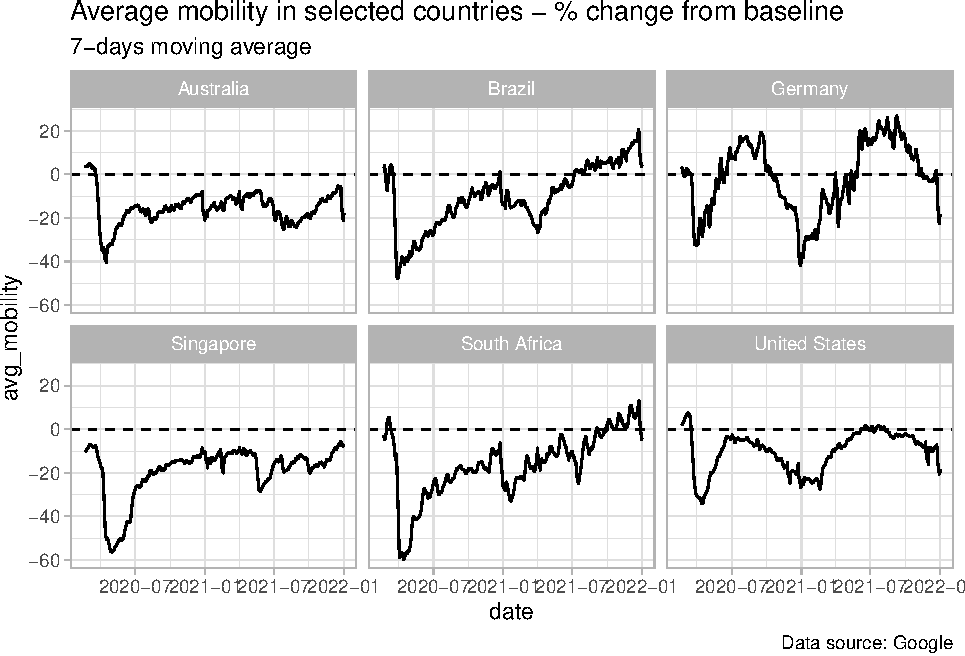
\includegraphics{RBook_files/figure-latex/ch1_chunk12-1.pdf}

\hypertarget{from-code-to-function}{%
\section{From code to function}\label{from-code-to-function}}

We have the complete code to import, prepare and visualize the data. Perhaps this analysis will become part of our routine or that of a stakeholder. And if that happens, it's very likely that we'll need to look at other countries. So a good practice in this case is to convert our code into a function.

Creating a function is highly recommended whenever we have a repeated action on a different set of arguments. Here, we can think of two arguments that we would like to change eventually: country and the window size of the rolling mean. Therefore our task is to gather all the code we have produced so far and to transform these two inputs into arguments of the function.

Note, however, that converting code into a function raises some issues. For example, when writing the code we used a vector to import data for the selected countries. It's not the most efficient approach, because each file has a significant size and thus the execution may be very slow. This is a truly concern when we're writing a function, because functions are most of the time used to loop over a large set of arguments -- many countries, for example. Hence, we would like to process this task in parallel rather than serially.

Surely we can perform this parallel processing inside the function, but I always prefer to keep things simpler and more transparent. This means to write a function to plot only a single country and, if necessary, we can use \texttt{purrr::map} to get as many countries as we want -- and (explicitly) in parallel.

Other minor yet important issue is that in a function we have to use the arguments as inputs everywhere, not only in obvious places. For example, when preparing the data we included a \texttt{ma7d} to the column names to indicate they were transformed into 7-days rolling mean. This label was also used in many actions later -- when computing the average mobility, in the plot subtitle, etc. Therefore, we need to ensure that this argument will be considered in those actions as well. To achieve this, we'll use \texttt{glue::glue()} function to create custom labels.

\begin{Shaded}
\begin{Highlighting}[]
\NormalTok{plot\_mobility }\OtherTok{\textless{}{-}} \ControlFlowTok{function}\NormalTok{(country\_code, ma\_window)\{}
  \FunctionTok{library}\NormalTok{(lubridate)}
  \FunctionTok{library}\NormalTok{(tidyverse)  }
  \FunctionTok{library}\NormalTok{(glue)}
  \CommentTok{\# Import data}
\NormalTok{  countries\_codes }\OtherTok{\textless{}{-}}\NormalTok{ country\_code}
\NormalTok{  years }\OtherTok{\textless{}{-}} \FunctionTok{seq}\NormalTok{(}\AttributeTok{from =} \DecValTok{2020}\NormalTok{,}
               \AttributeTok{to =}\NormalTok{ lubridate}\SpecialCharTok{::}\FunctionTok{year}\NormalTok{(}\FunctionTok{Sys.Date}\NormalTok{()), }
               \AttributeTok{by =} \DecValTok{1}\NormalTok{)}
\NormalTok{  google\_filenames }\OtherTok{\textless{}{-}} 
\NormalTok{    purrr}\SpecialCharTok{::}\FunctionTok{cross2}\NormalTok{(years, countries\_codes) }\SpecialCharTok{\%\textgreater{}\%} 
\NormalTok{    purrr}\SpecialCharTok{::}\FunctionTok{map\_chr}\NormalTok{(}\AttributeTok{.f =} \ControlFlowTok{function}\NormalTok{(x)\{}
\NormalTok{      x }\SpecialCharTok{\%\textgreater{}\%} 
\NormalTok{        glue}\SpecialCharTok{::}\FunctionTok{glue\_collapse}\NormalTok{(}\AttributeTok{sep =} \StringTok{\textquotesingle{}\_\textquotesingle{}}\NormalTok{) }\SpecialCharTok{\%\textgreater{}\%}
\NormalTok{        glue}\SpecialCharTok{::}\FunctionTok{glue}\NormalTok{(}\StringTok{\textquotesingle{}\_Region\_Mobility\_Report.csv\textquotesingle{}}\NormalTok{)}
\NormalTok{    \})}
\NormalTok{  mobility\_data }\OtherTok{\textless{}{-}} 
\NormalTok{    purrr}\SpecialCharTok{::}\FunctionTok{map\_dfr}\NormalTok{(}
      \AttributeTok{.x =}\NormalTok{ google\_filenames, }
      \AttributeTok{.f =} \ControlFlowTok{function}\NormalTok{(x)\{}
\NormalTok{        readr}\SpecialCharTok{::}\FunctionTok{read\_csv}\NormalTok{(}\FunctionTok{unz}\NormalTok{(}\StringTok{\textquotesingle{}data/Region\_Mobility\_Report\_CSVs.zip\textquotesingle{}}\NormalTok{, x))}
\NormalTok{      \})}
  \CommentTok{\# Prepare data}
\NormalTok{  mobility\_prep }\OtherTok{\textless{}{-}}\NormalTok{ mobility\_data }\SpecialCharTok{\%\textgreater{}\%} 
\NormalTok{    dplyr}\SpecialCharTok{::}\FunctionTok{filter}\NormalTok{(}\FunctionTok{is.na}\NormalTok{(sub\_region\_1)) }\SpecialCharTok{\%\textgreater{}\%}
\NormalTok{    dplyr}\SpecialCharTok{::}\FunctionTok{mutate}\NormalTok{(}\FunctionTok{across}\NormalTok{(}\FunctionTok{starts\_with}\NormalTok{(}\StringTok{\textquotesingle{}residential\textquotesingle{}}\NormalTok{), }\SpecialCharTok{\textasciitilde{}} \SpecialCharTok{{-}}\DecValTok{1}\SpecialCharTok{*}\NormalTok{.x)) }\SpecialCharTok{\%\textgreater{}\%}
\NormalTok{    dplyr}\SpecialCharTok{::}\FunctionTok{group\_by}\NormalTok{(country\_region) }\SpecialCharTok{\%\textgreater{}\%}
\NormalTok{    dplyr}\SpecialCharTok{::}\FunctionTok{arrange}\NormalTok{(date) }\SpecialCharTok{\%\textgreater{}\%} 
\NormalTok{    dplyr}\SpecialCharTok{::}\FunctionTok{mutate}\NormalTok{(}\FunctionTok{across}\NormalTok{(}\FunctionTok{ends\_with}\NormalTok{(}\StringTok{\textquotesingle{}baseline\textquotesingle{}}\NormalTok{), }\SpecialCharTok{\textasciitilde{}}\NormalTok{ RcppRoll}\SpecialCharTok{::}\FunctionTok{roll\_meanr}\NormalTok{(.x, ma\_window, }\AttributeTok{na.rm =} \ConstantTok{TRUE}\NormalTok{), }\AttributeTok{.names =} \StringTok{\textquotesingle{}\{.col\}\_ma\{ma\_window\}d\textquotesingle{}}\NormalTok{)) }\SpecialCharTok{\%\textgreater{}\%}
\NormalTok{    dplyr}\SpecialCharTok{::}\FunctionTok{ungroup}\NormalTok{() }\SpecialCharTok{\%\textgreater{}\%} 
\NormalTok{    dplyr}\SpecialCharTok{::}\FunctionTok{rowwise}\NormalTok{() }\SpecialCharTok{\%\textgreater{}\%} 
\NormalTok{    dplyr}\SpecialCharTok{::}\FunctionTok{mutate}\NormalTok{(}\AttributeTok{avg\_mobility =} \FunctionTok{mean}\NormalTok{(}\FunctionTok{c\_across}\NormalTok{(}\FunctionTok{ends\_with}\NormalTok{(}\FunctionTok{glue}\NormalTok{(}\StringTok{\textquotesingle{}ma\{ma\_window\}d\textquotesingle{}}\NormalTok{))), }\AttributeTok{na.rm =} \ConstantTok{TRUE}\NormalTok{)) }\SpecialCharTok{\%\textgreater{}\%}
\NormalTok{    dplyr}\SpecialCharTok{::}\FunctionTok{ungroup}\NormalTok{() }\SpecialCharTok{\%\textgreater{}\%} 
\NormalTok{    dplyr}\SpecialCharTok{::}\FunctionTok{select}\NormalTok{(date, country\_region, }\FunctionTok{ends\_with}\NormalTok{(}\StringTok{\textquotesingle{}baseline\textquotesingle{}}\NormalTok{), avg\_mobility) }
  \CommentTok{\# Output: plot}
\NormalTok{  mobility\_prep }\SpecialCharTok{\%\textgreater{}\%} 
    \FunctionTok{ggplot}\NormalTok{(}\FunctionTok{aes}\NormalTok{(}\AttributeTok{x =}\NormalTok{ date, }\AttributeTok{y =}\NormalTok{ avg\_mobility)) }\SpecialCharTok{+}
    \FunctionTok{geom\_line}\NormalTok{() }\SpecialCharTok{+}
    \FunctionTok{labs}\NormalTok{(}\AttributeTok{title =} \FunctionTok{glue}\NormalTok{(}\StringTok{\textquotesingle{}Average mobility in \{country\_code\} {-} \% change from baseline\textquotesingle{}}\NormalTok{),}
         \AttributeTok{subtitle =} \FunctionTok{glue}\NormalTok{(}\StringTok{\textquotesingle{}\{ma\_window\}{-}days moving average\textquotesingle{}}\NormalTok{),}
         \AttributeTok{caption =} \StringTok{\textquotesingle{}Data source: Google\textquotesingle{}}\NormalTok{) }\SpecialCharTok{+}
    \FunctionTok{geom\_hline}\NormalTok{(}\AttributeTok{yintercept =} \DecValTok{0}\NormalTok{, }\AttributeTok{linetype =} \DecValTok{2}\NormalTok{) }\SpecialCharTok{+}
    \FunctionTok{theme\_light}\NormalTok{()}
\NormalTok{\}}
\end{Highlighting}
\end{Shaded}

We can now use the function \texttt{plot\_mobility} to plot any country we want and with the desired window for the rolling mean.

\begin{Shaded}
\begin{Highlighting}[]
\FunctionTok{plot\_mobility}\NormalTok{(}\StringTok{\textquotesingle{}BR\textquotesingle{}}\NormalTok{, }\DecValTok{14}\NormalTok{)}
\end{Highlighting}
\end{Shaded}

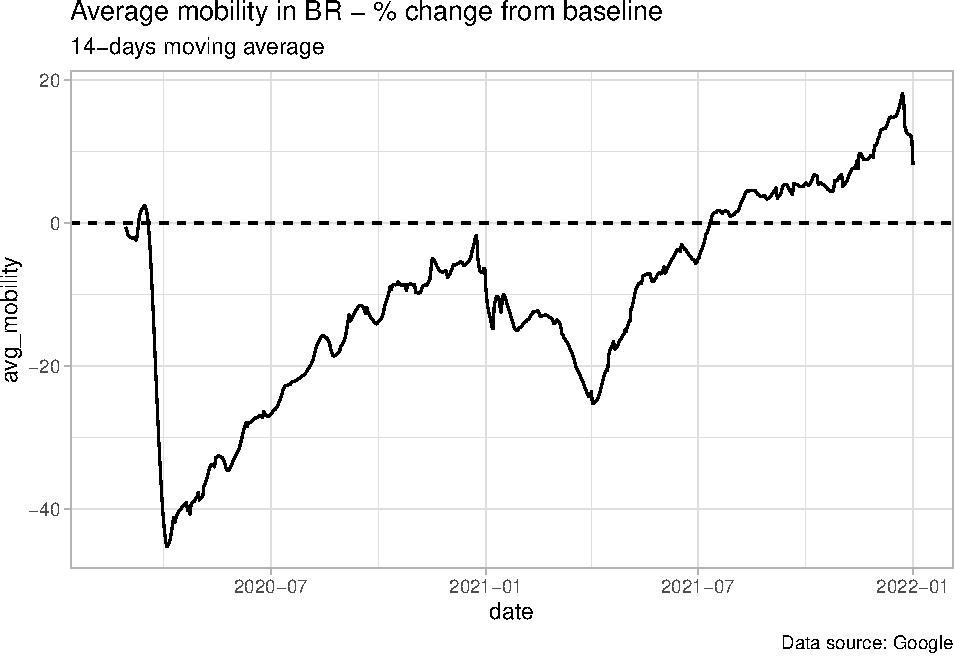
\includegraphics{RBook_files/figure-latex/ch01_chunk14-1.pdf}

Or we can use \texttt{purrr::map} and \texttt{gridExtra} to plot several countries.

\begin{Shaded}
\begin{Highlighting}[]
\NormalTok{countries }\OtherTok{\textless{}{-}} \FunctionTok{c}\NormalTok{(}\StringTok{\textquotesingle{}BR\textquotesingle{}}\NormalTok{, }\StringTok{\textquotesingle{}US\textquotesingle{}}\NormalTok{, }\StringTok{\textquotesingle{}FR\textquotesingle{}}\NormalTok{, }\StringTok{\textquotesingle{}DE\textquotesingle{}}\NormalTok{)}

\NormalTok{mobility\_countries }\OtherTok{\textless{}{-}}\NormalTok{ purrr}\SpecialCharTok{::}\FunctionTok{map}\NormalTok{(}\AttributeTok{.x =}\NormalTok{ countries, }\AttributeTok{.f =}\NormalTok{ plot\_mobility, }\DecValTok{14}\NormalTok{) }\SpecialCharTok{\%\textgreater{}\%} 
\NormalTok{  magrittr}\SpecialCharTok{::}\FunctionTok{set\_names}\NormalTok{(countries)}

\NormalTok{mobility\_countries[[}\StringTok{\textquotesingle{}DE\textquotesingle{}}\NormalTok{]]}
\end{Highlighting}
\end{Shaded}

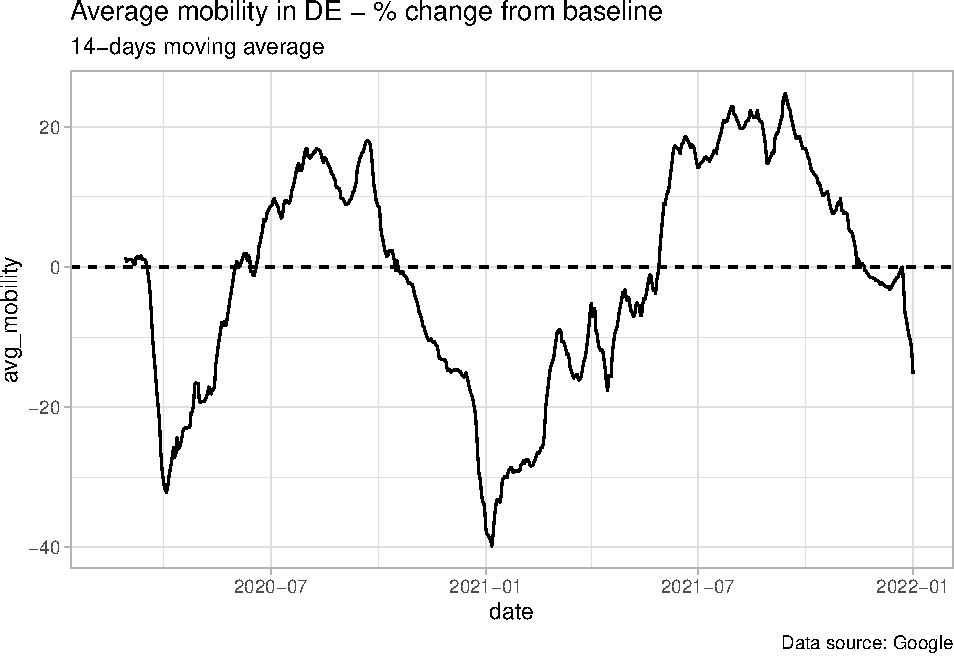
\includegraphics{RBook_files/figure-latex/ch01_chun15-1.pdf}

To finish up, we must keep in mind that a function that return a plot is not very flexible and maybe we should consider the output to be the processed data instead of the plot. This would enable us to customize the plot and to perform other analysis as well.

\hypertarget{owidCovid}{%
\chapter{Our World in Data COVID}\label{owidCovid}}

\hypertarget{importing-data-1}{%
\section{Importing data}\label{importing-data-1}}

In this Chapter, we'll turn to the COVID dataset from the Our World in Data project. It contains a complete set of variables related to COVID for a large number of countries. We can download it directly from the project's Github:

\begin{Shaded}
\begin{Highlighting}[]
\FunctionTok{library}\NormalTok{(tidyverse)}
\NormalTok{data\_url }\OtherTok{\textless{}{-}} \StringTok{\textquotesingle{}https://raw.githubusercontent.com/owid/covid{-}19{-}data/master/public/data/owid{-}covid{-}data.csv\textquotesingle{}}
\NormalTok{covid\_data }\OtherTok{\textless{}{-}}\NormalTok{ readr}\SpecialCharTok{::}\FunctionTok{read\_csv}\NormalTok{(data\_url)}
\end{Highlighting}
\end{Shaded}

\hypertarget{preparing-the-data-1}{%
\section{Preparing the data}\label{preparing-the-data-1}}

Suppose we're interested in producing a rank with the ten's most and least fully vaccinated countries in the world. At this time, fully vaccinated can be thought of as an individual who got two doses -- we won't consider booster doses. So our first task is to select the appropriate data on vaccinations. Using \texttt{dplyr::glimpse()} to check the variables in this dataset, we see three variables are of interest: \textbf{location, date and people\_fully\_vaccinated\_per\_hundred}.

Besides, it's likely that several countries don't have any data on vaccinations at all. This is the case of Vaticano, for example. We'd like to get rid of them, since they won't make part of our ranking. What we need, then, is a condition which returns \texttt{TRUE} only if a given location has any non-NA value.

\begin{Shaded}
\begin{Highlighting}[]
\NormalTok{vacc\_data }\OtherTok{\textless{}{-}}\NormalTok{ covid\_data }\SpecialCharTok{\%\textgreater{}\%} 
\NormalTok{  dplyr}\SpecialCharTok{::}\FunctionTok{select}\NormalTok{(location, }
\NormalTok{                date, }
\NormalTok{                people\_fully\_vaccinated\_per\_hundred) }\SpecialCharTok{\%\textgreater{}\%}   
\NormalTok{  dplyr}\SpecialCharTok{::}\FunctionTok{group\_by}\NormalTok{(location) }\SpecialCharTok{\%\textgreater{}\%} 
\NormalTok{  dplyr}\SpecialCharTok{::}\FunctionTok{filter}\NormalTok{(}\FunctionTok{any}\NormalTok{(}\SpecialCharTok{!}\FunctionTok{is.na}\NormalTok{(people\_fully\_vaccinated\_per\_hundred))) }\SpecialCharTok{\%\textgreater{}\%} 
\NormalTok{  dplyr}\SpecialCharTok{::}\FunctionTok{ungroup}\NormalTok{()}
\end{Highlighting}
\end{Shaded}

Since we only need the last figures for each country, we can filter the most recent observations.

\begin{Shaded}
\begin{Highlighting}[]
\NormalTok{vacc\_data\_last }\OtherTok{\textless{}{-}}\NormalTok{ vacc\_data }\SpecialCharTok{\%\textgreater{}\%} 
\NormalTok{  dplyr}\SpecialCharTok{::}\FunctionTok{group\_by}\NormalTok{(location) }\SpecialCharTok{\%\textgreater{}\%} 
\NormalTok{  dplyr}\SpecialCharTok{::}\FunctionTok{filter}\NormalTok{(date }\SpecialCharTok{==} \FunctionTok{max}\NormalTok{(date)) }\SpecialCharTok{\%\textgreater{}\%} 
\NormalTok{  dplyr}\SpecialCharTok{::}\FunctionTok{ungroup}\NormalTok{()}
\end{Highlighting}
\end{Shaded}

There's a problem here! For many countries the last day is filled with a \texttt{NA}, even though data is available for previous days. See, for example, the Netherlands. We know that 74.6\% of its population was vaccinated with two doses by 2021-12-12. But there's no data for the following seven days.

\begin{Shaded}
\begin{Highlighting}[]
\NormalTok{vacc\_data }\SpecialCharTok{\%\textgreater{}\%}
\NormalTok{  dplyr}\SpecialCharTok{::}\FunctionTok{filter}\NormalTok{(location }\SpecialCharTok{==} \StringTok{\textquotesingle{}Netherlands\textquotesingle{}}\NormalTok{) }\SpecialCharTok{\%\textgreater{}\%} 
\NormalTok{  dplyr}\SpecialCharTok{::}\FunctionTok{slice\_tail}\NormalTok{(}\AttributeTok{n =} \DecValTok{10}\NormalTok{)}
\end{Highlighting}
\end{Shaded}

\begin{verbatim}
## # A tibble: 10 x 3
##    location    date       people_fully_vaccinated_per_hundred
##    <chr>       <date>                                   <dbl>
##  1 Netherlands 2021-12-11                                NA  
##  2 Netherlands 2021-12-12                                74.6
##  3 Netherlands 2021-12-13                                NA  
##  4 Netherlands 2021-12-14                                NA  
##  5 Netherlands 2021-12-15                                NA  
##  6 Netherlands 2021-12-16                                NA  
##  7 Netherlands 2021-12-17                                NA  
##  8 Netherlands 2021-12-18                                NA  
##  9 Netherlands 2021-12-19                                NA  
## 10 Netherlands 2021-12-20                                NA
\end{verbatim}

We could think of different ways to retain the most recent non-NA observation in each country. But since the percentage of people vaccinated cannot decrease, it's entirely fair to carry this observation forward and consider it the most recent figure. How can we do it? The \texttt{fill()} function from the \texttt{tidyr} package is designed to fill missing values with the previous (default) or next non-NA value, the main argument being the columns we want to fill.

At this point, I'd like to call your attention for another powerful tool available in \texttt{dplyr} 1.0.0 or higher. Remember that we used \texttt{across} to select variables using the pattern in their names? The selection helper \texttt{where} does something similar, but instead of a name pattern it selects the variables for which a given function returns \texttt{TRUE}. For example, we know that the variable we want to fill is numeric. So we can use this condition to prevent us from writing it. It won't save us a lot of effort since we have only one variable with this condition here, but what if we had dozens?

\begin{Shaded}
\begin{Highlighting}[]
\NormalTok{vacc\_data\_last\_nonNA }\OtherTok{\textless{}{-}}\NormalTok{ vacc\_data }\SpecialCharTok{\%\textgreater{}\%} 
\NormalTok{  dplyr}\SpecialCharTok{::}\FunctionTok{group\_by}\NormalTok{(location) }\SpecialCharTok{\%\textgreater{}\%} 
\NormalTok{  dplyr}\SpecialCharTok{::}\FunctionTok{arrange}\NormalTok{(date) }\SpecialCharTok{\%\textgreater{}\%} 
\NormalTok{  tidyr}\SpecialCharTok{::}\FunctionTok{fill}\NormalTok{(}\FunctionTok{where}\NormalTok{(is.numeric)) }\SpecialCharTok{\%\textgreater{}\%} 
\NormalTok{  dplyr}\SpecialCharTok{::}\FunctionTok{filter}\NormalTok{(date }\SpecialCharTok{==} \FunctionTok{max}\NormalTok{(date)) }\SpecialCharTok{\%\textgreater{}\%} 
\NormalTok{  dplyr}\SpecialCharTok{::}\FunctionTok{ungroup}\NormalTok{()}
\end{Highlighting}
\end{Shaded}

We can check what happened to Netherlands' data for the last seven days. The last value from Dec 12th has been successfully carried forward up to Dec 19th. Now we're ready to create our ranking and then plot it to get e better sense of the inequality in the vaccination race between countries.

Notice I use \texttt{n()} inside the \texttt{dplyr::slice()} function. It's a great shortcut that can be used inside \texttt{dplyr} functions to avoid writing the number of rows in a data frame (or group). Also, note the use of \texttt{forcats::fct\_reorder}. The \texttt{forcats} package contains a lot of useful functions to handle factors and \texttt{fct\_reorder} is the one I use most. It reorder factor levels by sorting along another variable. In this case, as we are making a rank, it would be great if the locations were ordered by their position in the rank!

\begin{Shaded}
\begin{Highlighting}[]
\NormalTok{vacc\_rank }\OtherTok{\textless{}{-}}\NormalTok{ vacc\_data\_last\_nonNA }\SpecialCharTok{\%\textgreater{}\%} 
\NormalTok{  dplyr}\SpecialCharTok{::}\FunctionTok{mutate}\NormalTok{(}\AttributeTok{rank =}\NormalTok{ dplyr}\SpecialCharTok{::}\FunctionTok{dense\_rank}\NormalTok{(}\FunctionTok{desc}\NormalTok{(people\_fully\_vaccinated\_per\_hundred))) }\SpecialCharTok{\%\textgreater{}\%} 
\NormalTok{  dplyr}\SpecialCharTok{::}\FunctionTok{arrange}\NormalTok{(rank) }\SpecialCharTok{\%\textgreater{}\%} 
\NormalTok{  dplyr}\SpecialCharTok{::}\FunctionTok{slice}\NormalTok{(}\FunctionTok{c}\NormalTok{(}\DecValTok{1}\SpecialCharTok{:}\DecValTok{10}\NormalTok{, }\FunctionTok{n}\NormalTok{()}\SpecialCharTok{:}\NormalTok{(}\FunctionTok{n}\NormalTok{()}\SpecialCharTok{{-}}\DecValTok{9}\NormalTok{)))}

\NormalTok{vacc\_rank }\SpecialCharTok{\%\textgreater{}\%}
\NormalTok{  dplyr}\SpecialCharTok{::}\FunctionTok{mutate}\NormalTok{(}\AttributeTok{rank\_color =} \FunctionTok{if\_else}\NormalTok{(rank }\SpecialCharTok{\textless{}=} \DecValTok{10}\NormalTok{, }\StringTok{\textquotesingle{}good\textquotesingle{}}\NormalTok{, }\StringTok{\textquotesingle{}bad\textquotesingle{}}\NormalTok{)) }\SpecialCharTok{\%\textgreater{}\%} 
  \FunctionTok{ggplot}\NormalTok{(}\FunctionTok{aes}\NormalTok{(}\AttributeTok{x =}\NormalTok{ forcats}\SpecialCharTok{::}\FunctionTok{fct\_reorder}\NormalTok{(location, }\FunctionTok{desc}\NormalTok{(rank)), }
             \AttributeTok{y =}\NormalTok{ people\_fully\_vaccinated\_per\_hundred)) }\SpecialCharTok{+}
  \FunctionTok{geom\_col}\NormalTok{(}\FunctionTok{aes}\NormalTok{(}\AttributeTok{fill =}\NormalTok{ rank\_color)) }\SpecialCharTok{+}
  \FunctionTok{scale\_fill\_manual}\NormalTok{(}\AttributeTok{values =} \FunctionTok{c}\NormalTok{(}\StringTok{\textquotesingle{}red\textquotesingle{}}\NormalTok{, }\StringTok{\textquotesingle{}blue\textquotesingle{}}\NormalTok{)) }\SpecialCharTok{+}
  \FunctionTok{scale\_y\_continuous}\NormalTok{(}\AttributeTok{labels =} \ControlFlowTok{function}\NormalTok{(x) glue}\SpecialCharTok{::}\FunctionTok{glue}\NormalTok{(}\StringTok{\textquotesingle{}\{x\}\%\textquotesingle{}}\NormalTok{)) }\SpecialCharTok{+}
  \FunctionTok{geom\_text}\NormalTok{(}\FunctionTok{aes}\NormalTok{(}\AttributeTok{label =}\NormalTok{ glue}\SpecialCharTok{::}\FunctionTok{glue}\NormalTok{(}\StringTok{\textquotesingle{}\{people\_fully\_vaccinated\_per\_hundred\}\%\textquotesingle{}}\NormalTok{)), }
            \AttributeTok{nudge\_y =} \DecValTok{8}\NormalTok{) }\SpecialCharTok{+}
  \FunctionTok{theme\_light}\NormalTok{() }\SpecialCharTok{+}
  \FunctionTok{theme}\NormalTok{(}\AttributeTok{legend.position =} \StringTok{\textquotesingle{}none\textquotesingle{}}\NormalTok{) }\SpecialCharTok{+}
  \FunctionTok{coord\_flip}\NormalTok{() }\SpecialCharTok{+}
  \FunctionTok{labs}\NormalTok{(}\AttributeTok{title =} \StringTok{\textquotesingle{}Percentage of population fully vaccinated against COVID{-}19\textquotesingle{}}\NormalTok{,}
       \AttributeTok{x =} \StringTok{\textquotesingle{}\textquotesingle{}}\NormalTok{, }\AttributeTok{y =} \StringTok{\textquotesingle{}\textquotesingle{}}\NormalTok{)}
\end{Highlighting}
\end{Shaded}

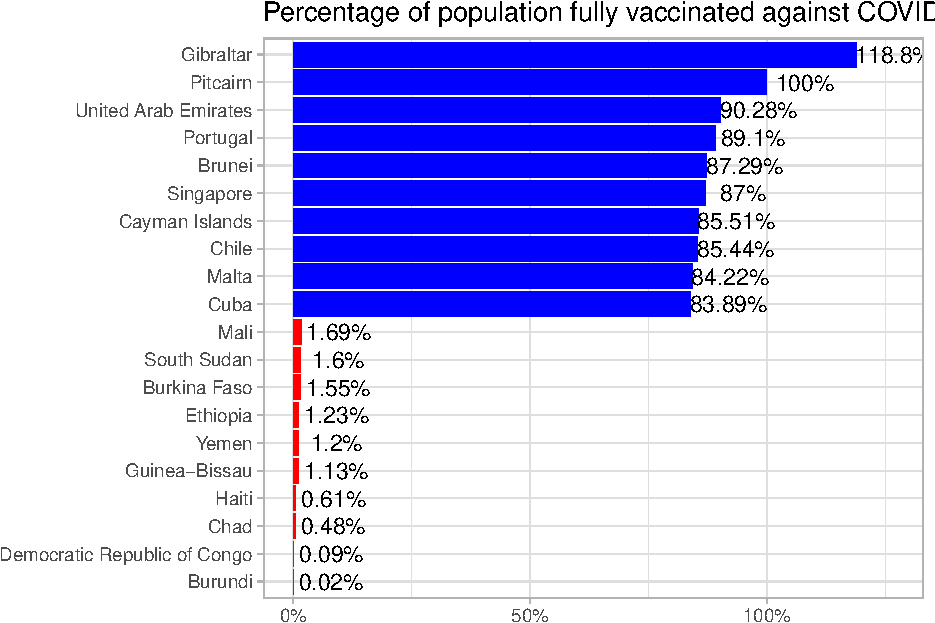
\includegraphics{RBook_files/figure-latex/ch4_chunk5-1.pdf}

  \bibliography{book.bib,packages.bib}

\end{document}
